% Options for packages loaded elsewhere
\PassOptionsToPackage{unicode}{hyperref}
\PassOptionsToPackage{hyphens}{url}
%
\documentclass[
  8pt,
  ignorenonframetext,
]{beamer}
\usepackage{pgfpages}
\setbeamertemplate{caption}[numbered]
\setbeamertemplate{caption label separator}{: }
\setbeamercolor{caption name}{fg=normal text.fg}
\beamertemplatenavigationsymbolsempty
% Prevent slide breaks in the middle of a paragraph
\widowpenalties 1 10000
\raggedbottom
\setbeamertemplate{part page}{
  \centering
  \begin{beamercolorbox}[sep=16pt,center]{part title}
    \usebeamerfont{part title}\insertpart\par
  \end{beamercolorbox}
}
\setbeamertemplate{section page}{
  \centering
  \begin{beamercolorbox}[sep=12pt,center]{part title}
    \usebeamerfont{section title}\insertsection\par
  \end{beamercolorbox}
}
\setbeamertemplate{subsection page}{
  \centering
  \begin{beamercolorbox}[sep=8pt,center]{part title}
    \usebeamerfont{subsection title}\insertsubsection\par
  \end{beamercolorbox}
}
\AtBeginPart{
  \frame{\partpage}
}
\AtBeginSection{
  \ifbibliography
  \else
    \frame{\sectionpage}
  \fi
}
\AtBeginSubsection{
  \frame{\subsectionpage}
}
\usepackage{amsmath,amssymb}
\usepackage{lmodern}
\usepackage{iftex}
\ifPDFTeX
  \usepackage[T1]{fontenc}
  \usepackage[utf8]{inputenc}
  \usepackage{textcomp} % provide euro and other symbols
\else % if luatex or xetex
  \usepackage{unicode-math}
  \defaultfontfeatures{Scale=MatchLowercase}
  \defaultfontfeatures[\rmfamily]{Ligatures=TeX,Scale=1}
\fi
% Use upquote if available, for straight quotes in verbatim environments
\IfFileExists{upquote.sty}{\usepackage{upquote}}{}
\IfFileExists{microtype.sty}{% use microtype if available
  \usepackage[]{microtype}
  \UseMicrotypeSet[protrusion]{basicmath} % disable protrusion for tt fonts
}{}
\makeatletter
\@ifundefined{KOMAClassName}{% if non-KOMA class
  \IfFileExists{parskip.sty}{%
    \usepackage{parskip}
  }{% else
    \setlength{\parindent}{0pt}
    \setlength{\parskip}{6pt plus 2pt minus 1pt}}
}{% if KOMA class
  \KOMAoptions{parskip=half}}
\makeatother
\usepackage{xcolor}
\newif\ifbibliography
\usepackage{color}
\usepackage{fancyvrb}
\newcommand{\VerbBar}{|}
\newcommand{\VERB}{\Verb[commandchars=\\\{\}]}
\DefineVerbatimEnvironment{Highlighting}{Verbatim}{commandchars=\\\{\}}
% Add ',fontsize=\small' for more characters per line
\usepackage{framed}
\definecolor{shadecolor}{RGB}{248,248,248}
\newenvironment{Shaded}{\begin{snugshade}}{\end{snugshade}}
\newcommand{\AlertTok}[1]{\textcolor[rgb]{0.94,0.16,0.16}{#1}}
\newcommand{\AnnotationTok}[1]{\textcolor[rgb]{0.56,0.35,0.01}{\textbf{\textit{#1}}}}
\newcommand{\AttributeTok}[1]{\textcolor[rgb]{0.77,0.63,0.00}{#1}}
\newcommand{\BaseNTok}[1]{\textcolor[rgb]{0.00,0.00,0.81}{#1}}
\newcommand{\BuiltInTok}[1]{#1}
\newcommand{\CharTok}[1]{\textcolor[rgb]{0.31,0.60,0.02}{#1}}
\newcommand{\CommentTok}[1]{\textcolor[rgb]{0.56,0.35,0.01}{\textit{#1}}}
\newcommand{\CommentVarTok}[1]{\textcolor[rgb]{0.56,0.35,0.01}{\textbf{\textit{#1}}}}
\newcommand{\ConstantTok}[1]{\textcolor[rgb]{0.00,0.00,0.00}{#1}}
\newcommand{\ControlFlowTok}[1]{\textcolor[rgb]{0.13,0.29,0.53}{\textbf{#1}}}
\newcommand{\DataTypeTok}[1]{\textcolor[rgb]{0.13,0.29,0.53}{#1}}
\newcommand{\DecValTok}[1]{\textcolor[rgb]{0.00,0.00,0.81}{#1}}
\newcommand{\DocumentationTok}[1]{\textcolor[rgb]{0.56,0.35,0.01}{\textbf{\textit{#1}}}}
\newcommand{\ErrorTok}[1]{\textcolor[rgb]{0.64,0.00,0.00}{\textbf{#1}}}
\newcommand{\ExtensionTok}[1]{#1}
\newcommand{\FloatTok}[1]{\textcolor[rgb]{0.00,0.00,0.81}{#1}}
\newcommand{\FunctionTok}[1]{\textcolor[rgb]{0.00,0.00,0.00}{#1}}
\newcommand{\ImportTok}[1]{#1}
\newcommand{\InformationTok}[1]{\textcolor[rgb]{0.56,0.35,0.01}{\textbf{\textit{#1}}}}
\newcommand{\KeywordTok}[1]{\textcolor[rgb]{0.13,0.29,0.53}{\textbf{#1}}}
\newcommand{\NormalTok}[1]{#1}
\newcommand{\OperatorTok}[1]{\textcolor[rgb]{0.81,0.36,0.00}{\textbf{#1}}}
\newcommand{\OtherTok}[1]{\textcolor[rgb]{0.56,0.35,0.01}{#1}}
\newcommand{\PreprocessorTok}[1]{\textcolor[rgb]{0.56,0.35,0.01}{\textit{#1}}}
\newcommand{\RegionMarkerTok}[1]{#1}
\newcommand{\SpecialCharTok}[1]{\textcolor[rgb]{0.00,0.00,0.00}{#1}}
\newcommand{\SpecialStringTok}[1]{\textcolor[rgb]{0.31,0.60,0.02}{#1}}
\newcommand{\StringTok}[1]{\textcolor[rgb]{0.31,0.60,0.02}{#1}}
\newcommand{\VariableTok}[1]{\textcolor[rgb]{0.00,0.00,0.00}{#1}}
\newcommand{\VerbatimStringTok}[1]{\textcolor[rgb]{0.31,0.60,0.02}{#1}}
\newcommand{\WarningTok}[1]{\textcolor[rgb]{0.56,0.35,0.01}{\textbf{\textit{#1}}}}
\usepackage{longtable,booktabs,array}
\usepackage{calc} % for calculating minipage widths
\usepackage{caption}
% Make caption package work with longtable
\makeatletter
\def\fnum@table{\tablename~\thetable}
\makeatother
\setlength{\emergencystretch}{3em} % prevent overfull lines
\providecommand{\tightlist}{%
  \setlength{\itemsep}{0pt}\setlength{\parskip}{0pt}}
\setcounter{secnumdepth}{-\maxdimen} % remove section numbering
\newlength{\cslhangindent}
\setlength{\cslhangindent}{1.5em}
\newlength{\csllabelwidth}
\setlength{\csllabelwidth}{3em}
\newlength{\cslentryspacingunit} % times entry-spacing
\setlength{\cslentryspacingunit}{\parskip}
\newenvironment{CSLReferences}[2] % #1 hanging-ident, #2 entry spacing
 {% don't indent paragraphs
  \setlength{\parindent}{0pt}
  % turn on hanging indent if param 1 is 1
  \ifodd #1
  \let\oldpar\par
  \def\par{\hangindent=\cslhangindent\oldpar}
  \fi
  % set entry spacing
  \setlength{\parskip}{#2\cslentryspacingunit}
 }%
 {}
\usepackage{calc}
\newcommand{\CSLBlock}[1]{#1\hfill\break}
\newcommand{\CSLLeftMargin}[1]{\parbox[t]{\csllabelwidth}{#1}}
\newcommand{\CSLRightInline}[1]{\parbox[t]{\linewidth - \csllabelwidth}{#1}\break}
\newcommand{\CSLIndent}[1]{\hspace{\cslhangindent}#1}
% type setting
% ------------------------------------------------------------------------------
\usepackage[german]{babel}     

% fonts
% ------------------------------------------------------------------------------
\usefonttheme{professionalfonts}

% slide title and horizontal line
% ------------------------------------------------------------------------------
\setbeamertemplate{frametitle}{%
    \vskip-30pt \color{black}\large%
    \begin{minipage}[b][23pt]{120mm}%
    \flushleft\insertframetitle%
    \end{minipage}%
}

\setbeamertemplate{headline}										
{
\vskip10pt\hfill\hspace{3.5mm} 										 
\vskip15pt\color{black}\rule{\textwidth}{0.4pt} 					 
}

% slide number
% ---------------------------------------------------------------
\setbeamertemplate{navigation symbols}{}
\setbeamertemplate{footline}
{
\vskip5pt
\vskip2pt
\makebox[123mm]{\hspace{7.5mm}
\hfill Wahrscheinlichkeitstheorie und Frequentistische Inferenz $\vert$ 
\copyright $ $ 2023 Dirk Ostwald CC BY 4.0 $\vert$ 
Folie \insertframenumber}
\vskip4pt
}

% block color scheme
% ------------------------------------------------------------------------------
% colors
\definecolor{white}{RGB}{255,255,255}
\definecolor{grey}{RGB}{235,235,235}
\definecolor{lightgrey}{RGB}{245,245,245}
\definecolor{LightBlue}{RGB}{220,220,255}
\definecolor{darkblue}{RGB}{51, 51, 153}

% definitions and theorems
\setbeamercolor{block title}{fg = black, bg = grey}
\setbeamercolor{block body}{fg = black, bg = lightgrey}

% general line spacing 
% ------------------------------------------------------------------------------
\linespread{1.3}

% local line spacing
% ------------------------------------------------------------------------------
\usepackage{setspace}

% colors
% -----------------------------------------------------------------------------
\usepackage{color}

% justified text
% ------------------------------------------------------------------------------
\usepackage{ragged2e}
\usepackage{etoolbox}
\apptocmd{\frame}{}{\justifying}{}

% bullet point lists
% -----------------------------------------------------------------------------
\setbeamertemplate{itemize item}[circle]
\setbeamertemplate{itemize subitem}[circle]
\setbeamertemplate{itemize subsubitem}[circle]
\setbeamercolor{itemize item}{fg = black}
\setbeamercolor{itemize subitem}{fg = black}
\setbeamercolor{itemize subsubitem}{fg = black}
\setbeamercolor{enumerate item}{fg = black}
\setbeamercolor{enumerate subitem}{fg = black}
\setbeamercolor{enumerate subsubitem}{fg = black}
\setbeamerfont{itemize/enumerate body}{}
\setbeamerfont{itemize/enumerate subbody}{size = \normalsize}
\setbeamerfont{itemize/enumerate subsubbody}{size = \normalsize}

% color links
% ------------------------------------------------------------------------------
\usepackage{hyperref}
\definecolor{urls}{RGB}{204,0,0}
\hypersetup{colorlinks, citecolor = darkblue, urlcolor = urls}


% additional math commands
% ------------------------------------------------------------------------------
\usepackage{bm}                                         
\newcommand{\niton}{\not\owns}
\newcommand{\ups} {\upsilon}


% text highlighting
% ------------------------------------------------------------------------------
\usepackage{soul}
\makeatletter
\let\HL\hl
\renewcommand\hl{%
  \let\set@color\beamerorig@set@color
  \let\reset@color\beamerorig@reset@color
  \HL}
\makeatother

% equation highlighting
% -----------------------------------------------------------------------------
\newcommand{\highlight}[2][yellow]{\mathchoice%
  {\colorbox{#1}{$\displaystyle#2$}}%
  {\colorbox{#1}{$\textstyle#2$}}%
  {\colorbox{#1}{$\scriptstyle#2$}}%
  {\colorbox{#1}{$\scriptscriptstyle#2$}}}%

% additional mathematical operators
% ------------------------------------------------------------------------------
\DeclareMathOperator*{\argmax}{arg\,max}
\DeclareMathOperator*{\argmin}{arg\,min}
\DeclareMathOperator*{\intinf}{\int_{-\infty}^{\infty}}
\ifLuaTeX
  \usepackage{selnolig}  % disable illegal ligatures
\fi
\IfFileExists{bookmark.sty}{\usepackage{bookmark}}{\usepackage{hyperref}}
\IfFileExists{xurl.sty}{\usepackage{xurl}}{} % add URL line breaks if available
\urlstyle{same} % disable monospaced font for URLs
\hypersetup{
  hidelinks,
  pdfcreator={LaTeX via pandoc}}

\author{}
\date{\vspace{-2.5em}}

\begin{document}

\begin{frame}[plain]{}
\protect\hypertarget{section}{}
\center

\begin{center}
\includegraphics[width=0.2\linewidth]{11_Abbildungen/wtfi_11_otto} \end{center}

\vspace{2mm}

\Large

Wahrscheinlichkeitstheorie und Frequentistische Inferenz \vspace{6mm}

\large

BSc Psychologie WiSe 2022/23

\vspace{6mm}
\normalsize

Prof.~Dr.~Dirk Ostwald
\end{frame}

\begin{frame}[plain]{}
\protect\hypertarget{section-1}{}
\vfill
\center
\huge

\textcolor{black}{(11) Konfidenzintervalle} \vfill
\end{frame}

\begin{frame}{}
\protect\hypertarget{section-2}{}
\begin{center}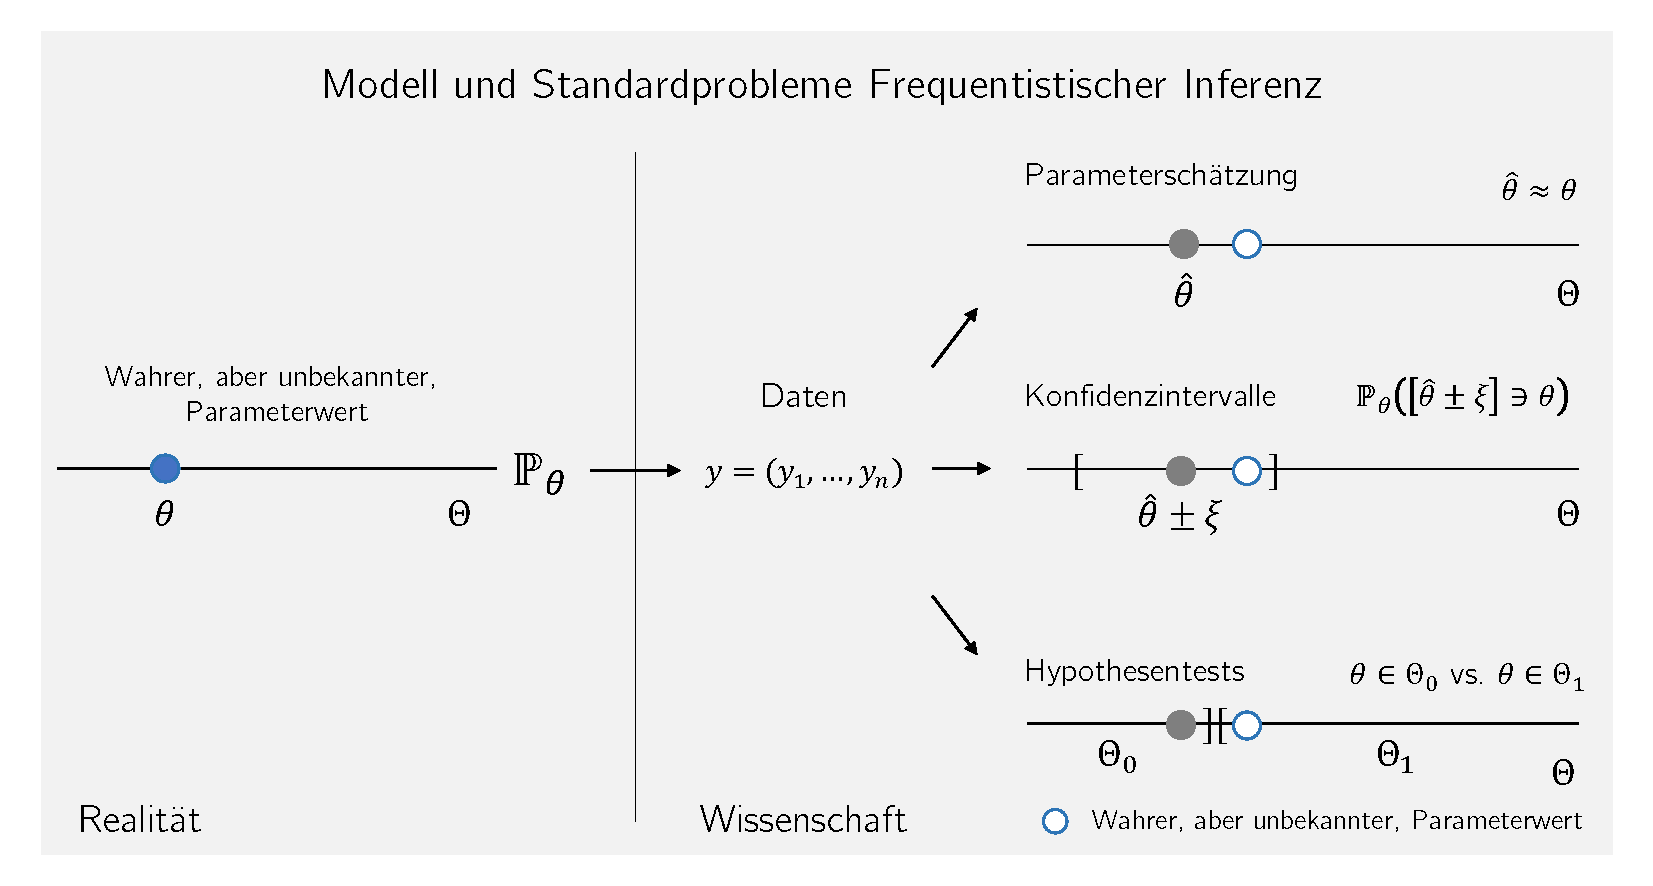
\includegraphics[width=1\linewidth]{11_Abbildungen/wtfi_11_frequentistische_inferenz} \end{center}
\end{frame}

\begin{frame}{}
\protect\hypertarget{section-3}{}
\begin{center}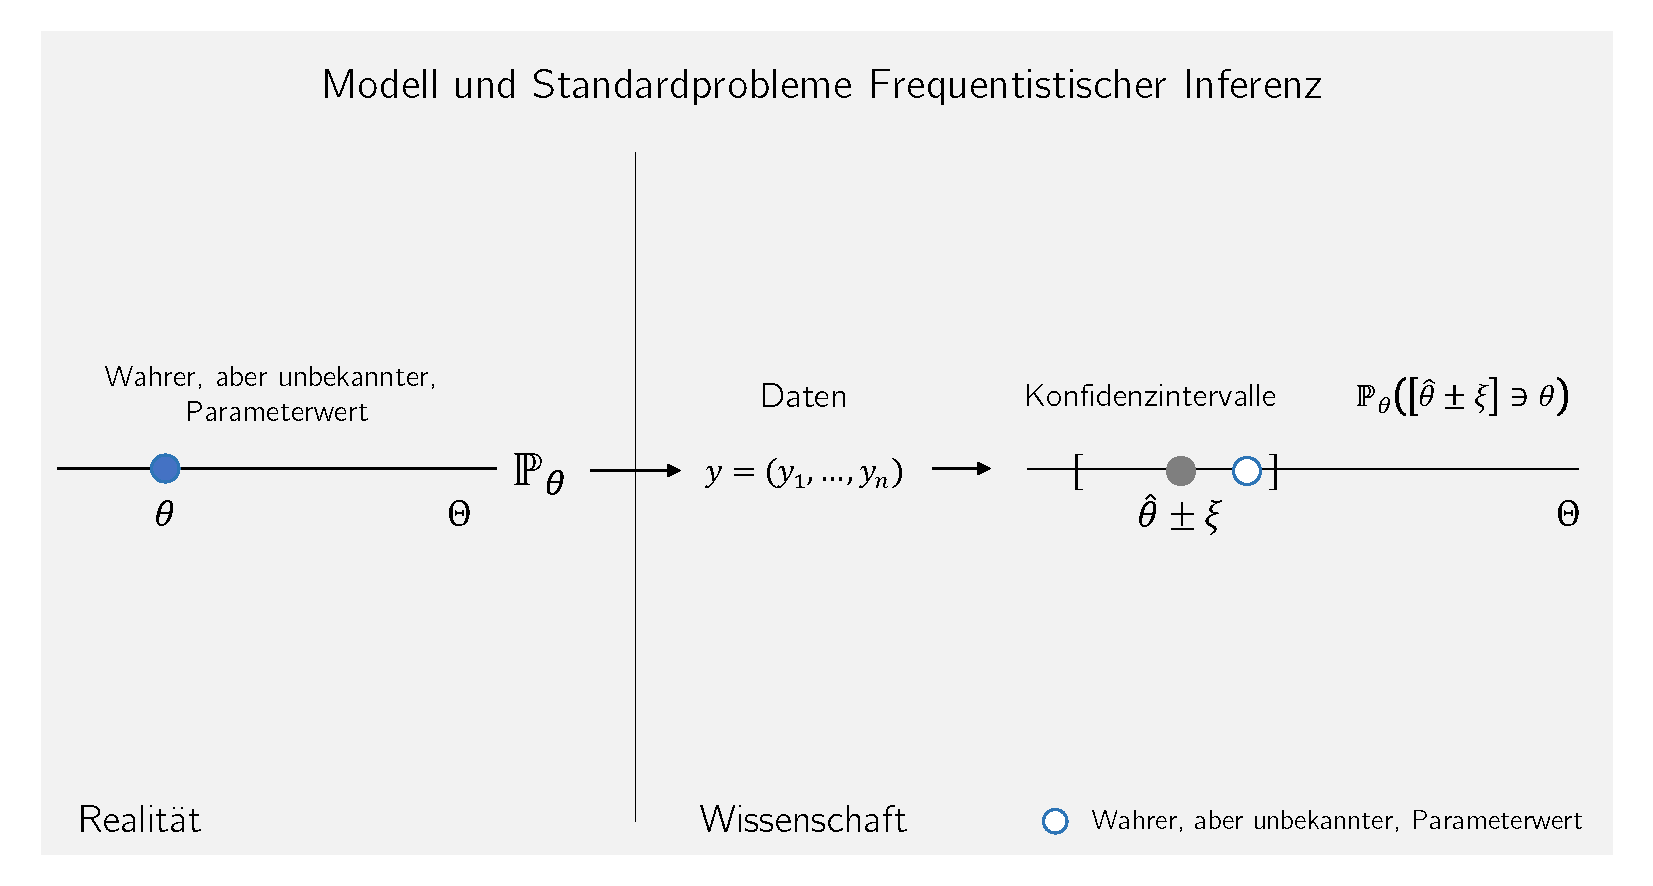
\includegraphics[width=1\linewidth]{11_Abbildungen/wtfi_11_frequentistische_inferenz_konfidenzintervalle} \end{center}
\end{frame}

\begin{frame}{}
\protect\hypertarget{section-4}{}
Standardannahmen Frequentistischer Inferenz

\footnotesize

\(\mathcal{M}\) sei ein statistisches Modell mit Stichprobe
\(\ups_1,...,\ups_n \sim p_\theta\). \textbf{Es wird angenommen, dass
ein konkret vorliegender Datensatz
\(y = (y_1,...,y_n) \in \mathbb{R}^n\) eine der möglichen Realisierungen
von \(\ups_1,...,\ups_n \sim p_\theta\) ist.} Aus Frequentistischer
Sicht kann man eine Studie unter gleichen Umständen unendlich oft
wiederholen und zu jedem Datensatz Schätzer oder Statistiken auswerten,
z.B. das Stichprobenmittel:

\footnotesize
\begin{itemize}
\item[] Datensatz (1) : $y^{(1)} = \left(y_1^{(1)}, y_2^{(1)}, ...,y_n^{(1)}\right)$
                        mit $\bar{y}^{(1)} = \frac{1}{n}\sum_{i=1}^n y_i^{(1)}$
\item[] Datensatz (2) : $y^{(2)} = \left(y_1^{(2)}, y_2^{(2)}, ...,y_n^{(2)}\right)$
                        mit $\bar{y}^{(2)} = \frac{1}{n}\sum_{i=1}^n y_i^{(2)}$
\item[] Datensatz (3) : $y^{(3)} = \left(y_1^{(3)}, y_2^{(3)}, ...,y_n^{(3)}\right)$
                        mit $\bar{y}^{(3)} = \frac{1}{n}\sum_{i=1}^n y_i^{(3)}$
\item[] Datensatz (4) : $y^{(4)} = \left(y_1^{(4)}, y_2^{(4)}, ...,y_n^{(4)}\right)$
                        mit $\bar{y}^{(4)} = \frac{1}{n}\sum_{i=1}^n y_i^{(4)}$
\item[] Datensatz (5) : $y^{(5)} = ...$
\end{itemize}

Um die Qualität statistischer Methoden zu beurteilen betrachtet die
Frequentistische Statistik deshalb die Wahrscheinlichkeitsverteilungen
von Schätzern und Statistiken unter Annahme von
\(\ups_1,...,\ups_n \sim p_\theta\). Was zum Beispiel ist die Verteilung
der \(\bar{y}^{(1)}\), \(\bar{y}^{(2)}\), \(\bar{y}^{(3)}\),
\(\bar{y}^{(4)}\), \ldots{} also die Verteilung der Zufallsvariable
\(\bar{\ups}\)?

Wenn eine statistische Methode im Sinne der Frequentistischen
Standardannahmen ``gut'' ist, dann heißt das also, dass sie bei häufiger
Anwendung ``im Mittel gut'' ist. Im Einzelfall, also im Normalfall nur
eines vorliegenden Datensatzes, kann sie auch ``schlecht'' sein.
\end{frame}

\begin{frame}{}
\protect\hypertarget{section-5}{}
\setstretch{2.7}
\large

Definition

Konfidenzintervall für den Erwartungswertparameter der Normalverteilung

Konfidenzintervall für den Varianzparameter der Normalverteilung

Anwendungsbeispiel

Selbstkontrollfragen
\end{frame}

\begin{frame}{}
\protect\hypertarget{section-6}{}
\setstretch{2.7}
\large

\textbf{Definition}

Konfidenzintervall für den Erwartungswertparameter der Normalverteilung

Konfidenzintervall für den Varianzparameter der Normalverteilung

Anwendungsbeispiel

Selbstkontrollfragen
\end{frame}

\begin{frame}{Definition}
\protect\hypertarget{definition}{}
\small
\begin{definition}[$\delta$-Konfidenzintervall]
\justifying
Es sei $\ups = \ups_1,...,\ups_n \sim p_\theta$ eine Stichprobe, $\delta \in \,]0,1[$,
und $G_u(\ups)$ und $G_o(\ups)$ seien zwei Statistiken. Dann ist ein
$\delta$-\textit{Konfidenzintervall} ein Intervall der Form $\kappa := [G_u, G_o]$, so dass
\begin{equation}
\mathbb{P}_\theta\left(\kappa \ni \theta\right) =
\mathbb{P}_\theta\left(G_u(\ups) \le \theta \le G_o(\ups) \right) =
\delta \mbox{ für alle } \theta \in \Theta \mbox{ gilt}.
\end{equation}
$\delta$ heißt das \textit{Konfidenzniveau} oder die \textit{Überdeckungswahrscheinlichkeit}
des Konfidenzintervalls. Die Statistiken $G_u(\ups)$ und $G_o(\ups)$ sind die unteren
und oberen Grenzen des Konfidenzintervalls.
\end{definition}

\footnotesize

Bemerkungen

\begin{itemize}
\tightlist
\item
  \(\theta\) ist fest, nicht zufällig, und unbekannt.
\item
  \(\kappa\) ist ein zufälliges Intervall, weil \(G_u(\ups)\) und
  \(G_o(\ups)\) Zufallsvariablen sind.
\item
  \(\kappa \ni \theta\) bedeutet \(\theta \in \kappa\), aber \(\kappa\)
  ist zufällig und steht deshalb vorn (cf.~\(\mathbb{P}(\xi = x)\)).
\item
  Ein \(\delta\)-Konfidenzintervall überdeckt den wahren Wert \(\theta\)
  mit Wahrscheinlichkeit \(\delta\).
\item
  Oft wird \(\delta = 0.95\) gewählt, also
  \textit{$95\%$-Konfidenzintervalle} betrachtet.
\end{itemize}
\end{frame}

\begin{frame}{Definition}
\protect\hypertarget{definition-1}{}
Zwei Interpretationen von \(\delta\)-Konfidenzintervallen

\small

\begin{enumerate}
[(1)]
\item
  \justifying  Wird ein Zufallsvorgang unter gleichen Umständen häufig
  wiederholt, so überdeckt das zugehörige \(\delta\)-Konfidenzintervall
  den wahren, aber unbekannten Parameterwert im langfristigen Mittel in
  \(\delta\cdot 100 \%\) der Fälle. Technischer ausgedrückt, für
  unabhängig und identisch realisierte Stichproben einer Verteilung mit
  wahrem, aber unbekannten, Parameter \(\theta\) überdeckt im
  langfristigen Mittel ein entsprechendes \(\delta\)-Konfidenzintervall
  \(\theta\) in \(\delta\cdot 100 \%\) aller Fälle.
\item
  Gegeben sei eine Menge von Zufallsvorgängen mit wahren, aber
  unbekannten, Parametern \(\theta_1,\theta_2,...\) und realisierte
  \(\delta\)-Konfidenzintervalle für eben jene Menge von wahren, aber
  unbekannten Parametern \(\theta_1,\theta_2,...\) Dann überdecken im
  langfristigen Mittel \(\delta\cdot 100 \%\) der Konfidenzintervalle
  den wahren, aber unbekannten, Wert \(\theta_i\) für \(i = 1,2,...\).
  Technischer ausgedrückt, für unabhängig realisierte Stichproben von
  Verteilungen mit wahren, aber unbekannten, Parametern
  \(\theta_1, \theta_2,...\) überdecken im langfristigen Mittel
  entsprechende \(\delta\)-Konfidenzintervalle \(\theta_i\) für
  \(i = 1,2,...\) in \(\delta\cdot 100 \%\) aller Fälle.
\end{enumerate}

Wir demonstrieren im Folgenden beide Interpretationen mithilfe von
Simulationen.
\end{frame}

\begin{frame}{Definition}
\protect\hypertarget{definition-2}{}
\setstretch{1.6}

Allgemeine Konstruktion von Konfidenzintervallen

\begin{enumerate}
[(1)]
\tightlist
\item
  Definition des statistischen Modells
\item
  Definition der Konfidenzintervallstatistik
\item
  Analyse der Verteilung der Konfidenzintervallstatistik
\item
  Etablierung der Konfidenzbedingung
\item
  Definition des Konfidenzintervalls
\end{enumerate}

\normalsize

Beispiele

\begin{enumerate}
[(1)]
\tightlist
\item
  Konfidenzintervall für den Erwartungswertparameter der
  Normalverteilung
\item
  Konfidenzintervall für den Varianzparameter der Normalverteilung
\end{enumerate}
\end{frame}

\begin{frame}{}
\protect\hypertarget{section-7}{}
\setstretch{2.7}
\large

Definition

\normalsize

\textbf{Konfidenzintervall für den Erwartungswertparameter der
Normalverteilung}

\large

Konfidenzintervall für den Varianzparameter der Normalverteilung

Anwendungsbeispiel

Selbstkontrollfragen
\end{frame}

\begin{frame}{Konfidenzintervall für den Erwartungswertparameter der
Normalverteilung}
\protect\hypertarget{konfidenzintervall-fuxfcr-den-erwartungswertparameter-der-normalverteilung}{}
\noindent (1) Definition des statistischen Modells

\small

Es sei \(\ups := \ups_1,...,\ups_n \sim N(\mu,\sigma^2)\) eine
Stichprobe mit unbekannten Parametern \(\mu\) und \(\sigma^2 > 0\). Wir
entwickeln ein \(\delta\)-Konfidenzintervall für den
Erwartungswertparameter \(\mu\). \vspace{2mm}

\normalsize

\noindent (2) Definition der Statistik \small

Wir betrachten die \(T\)-Konfidenzintervallstatistik \begin{equation}
T := \frac{\sqrt{n}}{S}(\bar{\ups} - \mu) \mbox{ mit } \bar{\ups} := \frac{1}{n}\sum_{i=1}^n \ups_i \mbox{  und } S := \sqrt{\frac{1}{n-1}\sum_{i=1}^n(\ups_i - \bar{\ups})^2}.
\end{equation}

\normalsize

\noindent (3) Analyse der Verteilung der Konfidenzintervallstatistik

\small

Für die \(T\)-Konfidenzintervallstatistik gilt \(T \sim t(n - 1)\), die
\(T\)-Konfidenzintervallstatistik ist also eine \(t\)-verteilte
Zufallsvariable mit Freiheitsgradparameter \(n-1\). Wir verzichten auf
einen Beweis. Die \(T\)-Konfidenzintervallstatistik ist eine Funktion
der Stichprobe \(\ups_1,...,\ups_n\) (via \(\bar{\ups}\) und \(S\)),
während ihre Verteilung weder von \(\mu\) noch von \(\sigma^2\) abhängt.
Wir bezeichnen die die WDF einer \(t\)-verteilten Zufallvariable mit
\(t\), die KVF einer \(t\)-verteilten Zufallvariable mit \(\Psi\) und
die inverse KVF einer \(t\)-verteilten Zufallvariable mit \(\Psi^{-1}\).
\end{frame}

\begin{frame}[fragile]{Konfidenzintervall für den
Erwartungswertparameter der Normalverteilung}
\protect\hypertarget{konfidenzintervall-fuxfcr-den-erwartungswertparameter-der-normalverteilung-1}{}
\normalsize

\noindent (3) Analyse der Verteilung der Konfidenzintervallstatistik
(fortgeführt) \vspace{2mm}

\tiny
\setstretch{1.1}

\begin{Shaded}
\begin{Highlighting}[]
\CommentTok{\# Modellformulierung}
\NormalTok{mu      }\OtherTok{=} \DecValTok{10}                                          \CommentTok{\# w.a.u. Erwartungswertparameter}
\NormalTok{sigsqr  }\OtherTok{=} \DecValTok{4}                                           \CommentTok{\# wahrer bekannter Varianzparameter}
\NormalTok{n       }\OtherTok{=} \DecValTok{12}                                          \CommentTok{\# Stichprobengroesse}
\NormalTok{ns      }\OtherTok{=} \FloatTok{1e4}                                         \CommentTok{\# Anzahl Stichprobenrealisierungen}
\NormalTok{res     }\OtherTok{=} \FloatTok{1e3}                                         \CommentTok{\# Ausgangsraumaufloesung}

\CommentTok{\# analytische Definitionen und Resultate}
\NormalTok{y\_1     }\OtherTok{=} \FunctionTok{seq}\NormalTok{(}\DecValTok{3}\NormalTok{,}\DecValTok{17}\NormalTok{,}\AttributeTok{len =}\NormalTok{ res)                         }\CommentTok{\# y\_1 Raum}
\NormalTok{t       }\OtherTok{=} \FunctionTok{seq}\NormalTok{(}\SpecialCharTok{{-}}\DecValTok{4}\NormalTok{,}\DecValTok{4}\NormalTok{,}\AttributeTok{len =}\NormalTok{ res)                         }\CommentTok{\# t Raum}
\NormalTok{p\_y\_1   }\OtherTok{=} \FunctionTok{dnorm}\NormalTok{(y\_1,mu,}\FunctionTok{sqrt}\NormalTok{(sigsqr))                  }\CommentTok{\# y\_1 WDF}
\NormalTok{p\_y\_bar }\OtherTok{=} \FunctionTok{dnorm}\NormalTok{(y\_1,mu,}\FunctionTok{sqrt}\NormalTok{(sigsqr}\SpecialCharTok{/}\NormalTok{n))                }\CommentTok{\# y\_bar WDF}
\NormalTok{p\_t     }\OtherTok{=} \FunctionTok{dt}\NormalTok{(t,n}\DecValTok{{-}1}\NormalTok{)                                   }\CommentTok{\# t WDF}

\CommentTok{\# Simulation}
\NormalTok{y\_i     }\OtherTok{=} \FunctionTok{rep}\NormalTok{(}\ConstantTok{NaN}\NormalTok{,ns)                                 }\CommentTok{\# y\_1 Array}
\NormalTok{y\_bar   }\OtherTok{=} \FunctionTok{rep}\NormalTok{(}\ConstantTok{NaN}\NormalTok{,ns)                                 }\CommentTok{\# \textbackslash{}bar\{y\} Array}
\NormalTok{Tee     }\OtherTok{=} \FunctionTok{rep}\NormalTok{(}\ConstantTok{NaN}\NormalTok{,ns)                                 }\CommentTok{\# T Array}
\ControlFlowTok{for}\NormalTok{(s }\ControlFlowTok{in} \DecValTok{1}\SpecialCharTok{:}\NormalTok{ns)\{                                       }\CommentTok{\# Simulationsiterationen}
\NormalTok{  y         }\OtherTok{=} \FunctionTok{rnorm}\NormalTok{(n,mu,}\FunctionTok{sqrt}\NormalTok{(sigsqr))                }\CommentTok{\# Stichprobenrealisierung}
\NormalTok{  y\_i[s]    }\OtherTok{=}\NormalTok{ y[}\DecValTok{1}\NormalTok{]                                    }\CommentTok{\# \textbackslash{}ups\_i}
\NormalTok{  y\_bar[s]  }\OtherTok{=} \FunctionTok{mean}\NormalTok{(y)                                 }\CommentTok{\# Stichprobenmittelrealisierung}
\NormalTok{  Tee[s]    }\OtherTok{=} \FunctionTok{sqrt}\NormalTok{(n)}\SpecialCharTok{*}\NormalTok{((y\_bar[s] }\SpecialCharTok{{-}}\NormalTok{ mu)}\SpecialCharTok{/}\FunctionTok{sqrt}\NormalTok{(}\FunctionTok{var}\NormalTok{(y)))  }\CommentTok{\# T{-}Statistik Realisierung}
\NormalTok{\}}
\end{Highlighting}
\end{Shaded}
\end{frame}

\begin{frame}{Konfidenzintervall für den Erwartungswertparameter der
Normalverteilung}
\protect\hypertarget{konfidenzintervall-fuxfcr-den-erwartungswertparameter-der-normalverteilung-2}{}
\normalsize

\noindent (3) Analyse der Verteilung der Konfidenzintervallstatistik
(fortgeführt)

\vfill

\begin{center}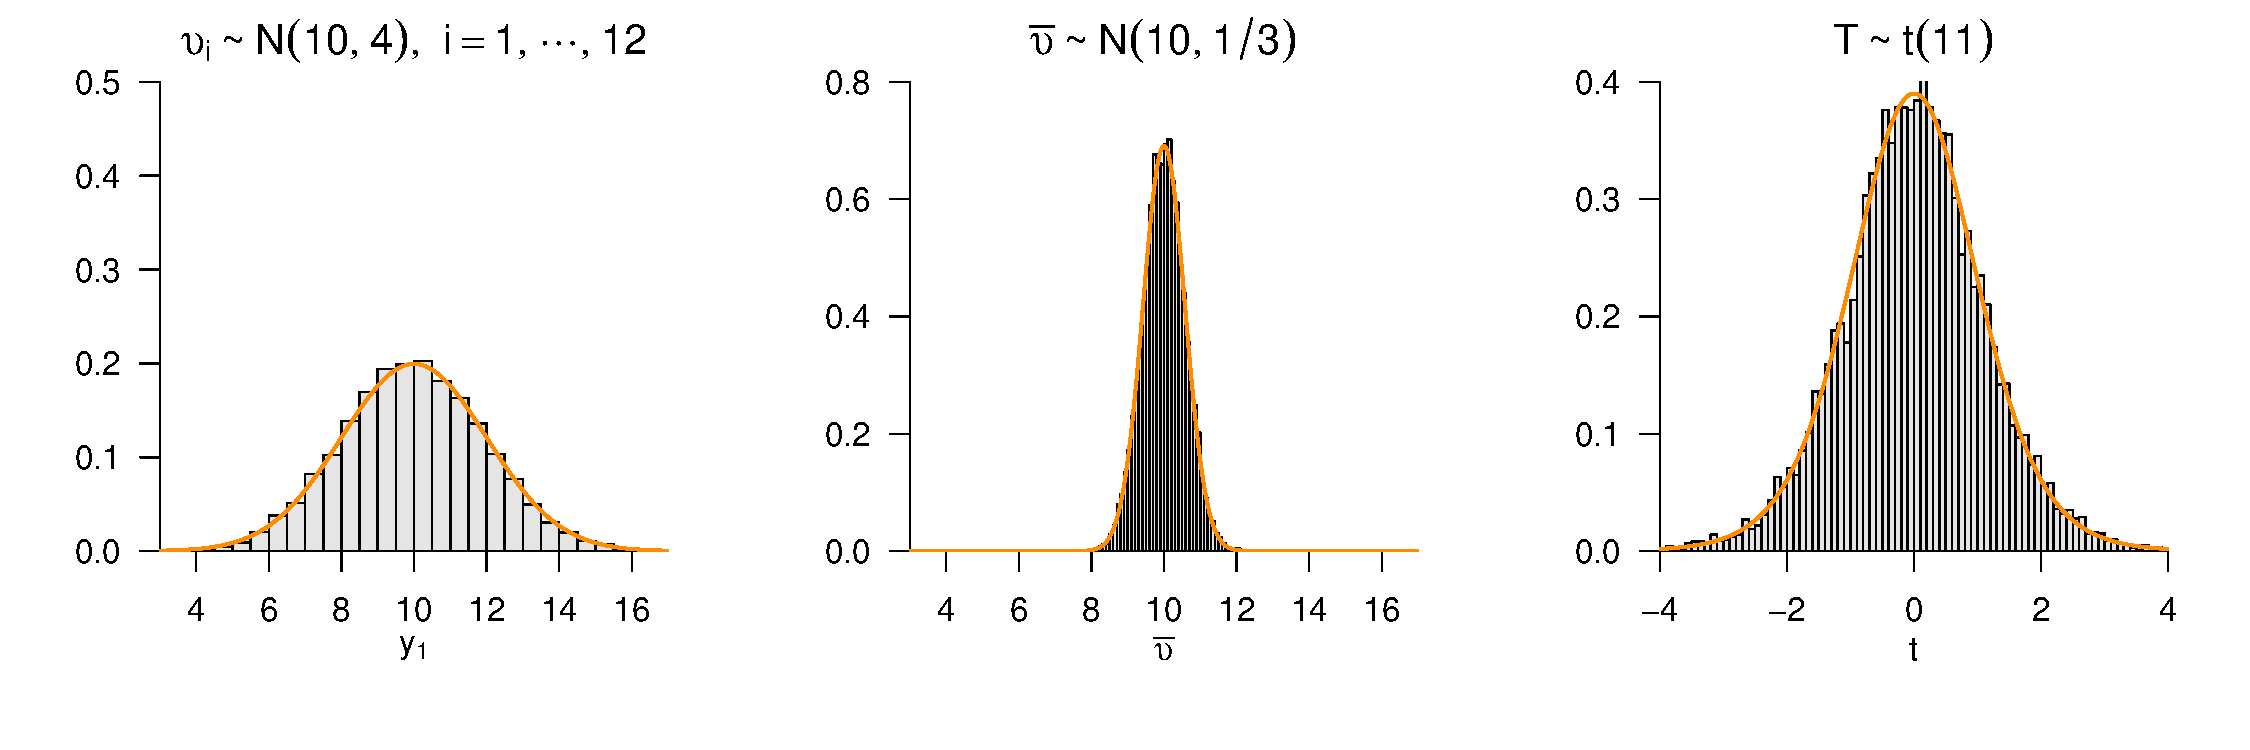
\includegraphics[width=1\linewidth]{11_Abbildungen/wtfi_11_t_statistik} \end{center}
\vfill
\end{frame}

\begin{frame}{Konfidenzintervall für den Erwartungswertparameter der
Normalverteilung}
\protect\hypertarget{konfidenzintervall-fuxfcr-den-erwartungswertparameter-der-normalverteilung-3}{}
\noindent (4) Etablierung der Konfidenzbedingung

\small

Für \(\delta \in ]0,1[\) seien \begin{equation}
t_1 := \Psi^{-1}\left(\frac{1 - \delta}{2}; n - 1\right)
\mbox{ und }
t_2 := \Psi^{-1}\left(\frac{1 + \delta}{2}; n-1\right)
\end{equation} Es gilt dann \((1 + \delta)/2 - (1 - \delta)/2 = \delta\)
und zum Beispiel gilt für \(n = 5\) und \(\delta = 0.95\),
\(t_1 = \Psi^{-1}(0.025;4) = -2.57\) und
\(t_2 = \Psi^{-1}(0.975;4) = 2.57\). Weiterhin gilt mit der Symmetrie
von \(t(n-1)\), \(t_1 = - t_2\). Es gilt hier also per Definition
\(\mathbb{P}\left(-t_2 \le T \le t_2 \right) = \delta\).

\vspace{2mm}

\begin{center}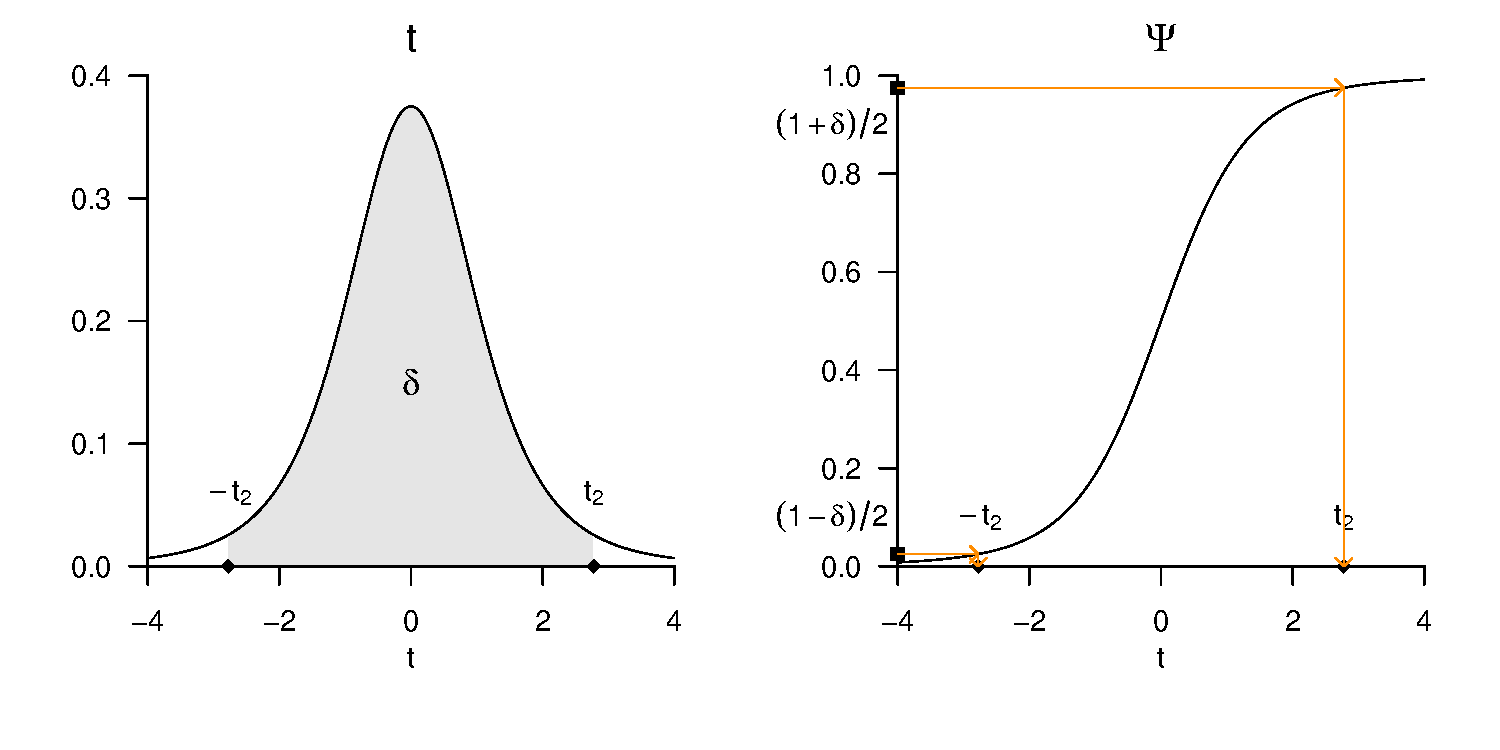
\includegraphics[width=0.8\linewidth]{11_Abbildungen/wtfi_11_ki_t_konfidenzbedingung} \end{center}
\end{frame}

\begin{frame}{Konfidenzintervall für den Erwartungswertparameter der
Normalverteilung}
\protect\hypertarget{konfidenzintervall-fuxfcr-den-erwartungswertparameter-der-normalverteilung-4}{}
\noindent (4) Etablierung der Konfidenzbedingung (fortgeführt)

\small

Mit der Definition von \(t_2\) wie oben folgt dann aber \footnotesize
\begin{align}
\begin{split}
\delta
& =
\mathbb{P}\left(-t_2 \le T \le t_2 \right)                                                                          \\
& =
\mathbb{P}\left(-t_2 \le \frac{\sqrt{n}}{S}(\bar{\ups} - \mu) \le t_2 \right)                                       \\
& =
\mathbb{P}\left(-\frac{S}{\sqrt{n}}t_2 \le \bar{\ups} - \mu \le \frac{S}{\sqrt{n}}t_2 \right)                   \\
& =
\mathbb{P}\left(-\bar{\ups} -\frac{S}{\sqrt{n}}t_2 \le - \mu \le - \bar{\ups} + \frac{S}{\sqrt{n}}t_2 \right)   \\
& =
\mathbb{P}\left(\bar{\ups} + \frac{S}{\sqrt{n}}t_2 \ge \mu \ge \bar{\ups} - \frac{S}{\sqrt{n}}t_2 \right)       \\
& =
\mathbb{P}\left(\bar{\ups} - \frac{S}{\sqrt{n}}t_2 \le \mu \le \bar{\ups} + \frac{S}{\sqrt{n}}t_2 \right)       \\
& =
\mathbb{P}\left(\left[\bar{\ups} - \frac{S}{\sqrt{n}}t_2, \bar{\ups} + \frac{S}{\sqrt{n}}t_2\right] \ni \mu \right).        \\
\end{split}
\end{align} \small Wir können nun das gesuchte Konfidenzintervall
definieren.
\end{frame}

\begin{frame}{Konfidenzintervall für den Erwartungswertparameter der
Normalverteilung}
\protect\hypertarget{konfidenzintervall-fuxfcr-den-erwartungswertparameter-der-normalverteilung-5}{}
\noindent(5) Definition des Konfidenzintervalls \small

Es sei \(\ups_1,...,\ups_n \sim N(\mu,\sigma^2)\) mit unbekannten
Parametern \(\mu\) und \(\sigma^2\), es sei \(\delta \in ]0,1[\) und es
sei \begin{equation}
t_\delta := \Psi^{-1}\left(\frac{1+\delta}{2}; n - 1\right).
\end{equation} Definiere \begin{equation}
\kappa :=
\left[\bar{\ups} - \frac{S}{\sqrt{n}}t_\delta,
\bar{\ups} + \frac{S}{\sqrt{n}}t_\delta\right].
\end{equation} Dann gilt wie oben gezeigt \begin{equation}
\mathbb{P}(\kappa \ni \mu) = \delta.
\end{equation} Damit ist \(\kappa\) ein \(\delta\)-Konfidenzintervall
für \(\mu\).

Man beachte, dass \(\kappa\) ein zufälliges Intervall ist, weil
\(\bar{\ups}\) und \(S\) Zufallsvariablen sind.
\end{frame}

\begin{frame}[fragile]{Konfidenzintervall für den
Erwartungswertparameter der Normalverteilung}
\protect\hypertarget{konfidenzintervall-fuxfcr-den-erwartungswertparameter-der-normalverteilung-6}{}
\noindent(5) Definition des Konfidenzintervalls (fortgeführt)

\small

Simulation der ersten Interpretation eines Konfidenzintervalls
\vspace{2mm}

\setstretch{1}
\footnotesize

\begin{Shaded}
\begin{Highlighting}[]
\CommentTok{\# Modellformulierung}
\FunctionTok{set.seed}\NormalTok{(}\DecValTok{1}\NormalTok{)                                        }\CommentTok{\# random number generator seed}
\NormalTok{mu      }\OtherTok{=} \DecValTok{2}                                        \CommentTok{\# w.a.u. Erwartungswertparameter}
\NormalTok{sigsqr  }\OtherTok{=} \DecValTok{1}                                        \CommentTok{\# w.a.u. Varianzparameter}
\NormalTok{sigma   }\OtherTok{=} \FunctionTok{sqrt}\NormalTok{(sigsqr)                             }\CommentTok{\# w.a.u. St.Abweichungsparameter}
\NormalTok{n       }\OtherTok{=} \DecValTok{12}                                       \CommentTok{\# Stichprobengroesse}
\NormalTok{delta   }\OtherTok{=} \FloatTok{0.95}                                     \CommentTok{\# Konfidenzbedingung}
\NormalTok{t\_delta }\OtherTok{=} \FunctionTok{qt}\NormalTok{((}\DecValTok{1}\SpecialCharTok{+}\NormalTok{delta)}\SpecialCharTok{/}\DecValTok{2}\NormalTok{,n}\DecValTok{{-}1}\NormalTok{)                      }\CommentTok{\# \textbackslash{}Psi\^{}{-}1((\textbackslash{}delta + 1)/2, n{-}1)}

\CommentTok{\# Simulation}
\NormalTok{ns      }\OtherTok{=} \FloatTok{1e2}                                      \CommentTok{\# Anzahl Simulationen}
\NormalTok{y\_bar   }\OtherTok{=} \FunctionTok{rep}\NormalTok{(}\ConstantTok{NaN}\NormalTok{,ns)                              }\CommentTok{\# Stichprobenmittelarray}
\NormalTok{S       }\OtherTok{=} \FunctionTok{rep}\NormalTok{(}\ConstantTok{NaN}\NormalTok{,ns)                              }\CommentTok{\# St.Abweichungsarray}
\NormalTok{kappa   }\OtherTok{=} \FunctionTok{matrix}\NormalTok{(}\FunctionTok{rep}\NormalTok{(}\ConstantTok{NaN}\NormalTok{,}\DecValTok{2}\SpecialCharTok{*}\NormalTok{ns), }\AttributeTok{ncol =} \DecValTok{2}\NormalTok{)          }\CommentTok{\# Konfidenzintervallarray}
\ControlFlowTok{for}\NormalTok{(i }\ControlFlowTok{in} \DecValTok{1}\SpecialCharTok{:}\NormalTok{ns)\{}
\NormalTok{   y          }\OtherTok{=} \FunctionTok{rnorm}\NormalTok{(n,mu,sigma)                  }\CommentTok{\# Stichprobenrealisierung}
\NormalTok{   y\_bar[i]   }\OtherTok{=} \FunctionTok{mean}\NormalTok{(y)                            }\CommentTok{\# Stichprobenmittel}
\NormalTok{   S[i]       }\OtherTok{=} \FunctionTok{sd}\NormalTok{(y)                              }\CommentTok{\# Stichprobenstandardabweichung}
\NormalTok{   kappa[i,}\DecValTok{1}\NormalTok{] }\OtherTok{=}\NormalTok{ y\_bar[i] }\SpecialCharTok{{-}}\NormalTok{ (S[i]}\SpecialCharTok{/}\FunctionTok{sqrt}\NormalTok{(n))}\SpecialCharTok{*}\NormalTok{t\_delta  }\CommentTok{\# untere KI Grenze}
\NormalTok{   kappa[i,}\DecValTok{2}\NormalTok{] }\OtherTok{=}\NormalTok{ y\_bar[i] }\SpecialCharTok{+}\NormalTok{ (S[i]}\SpecialCharTok{/}\FunctionTok{sqrt}\NormalTok{(n))}\SpecialCharTok{*}\NormalTok{t\_delta  }\CommentTok{\# obere KI Grenze}
\NormalTok{\}}
\end{Highlighting}
\end{Shaded}
\end{frame}

\begin{frame}{Konfidenzintervall für den Erwartungswertparameter der
Normalverteilung}
\protect\hypertarget{konfidenzintervall-fuxfcr-den-erwartungswertparameter-der-normalverteilung-7}{}
\noindent(5) Definition des Konfidenzintervalls (fortgeführt)

\small

Simulation der ersten Interpretation eines Konfidenzintervalls

\vspace{3mm}

\begin{center}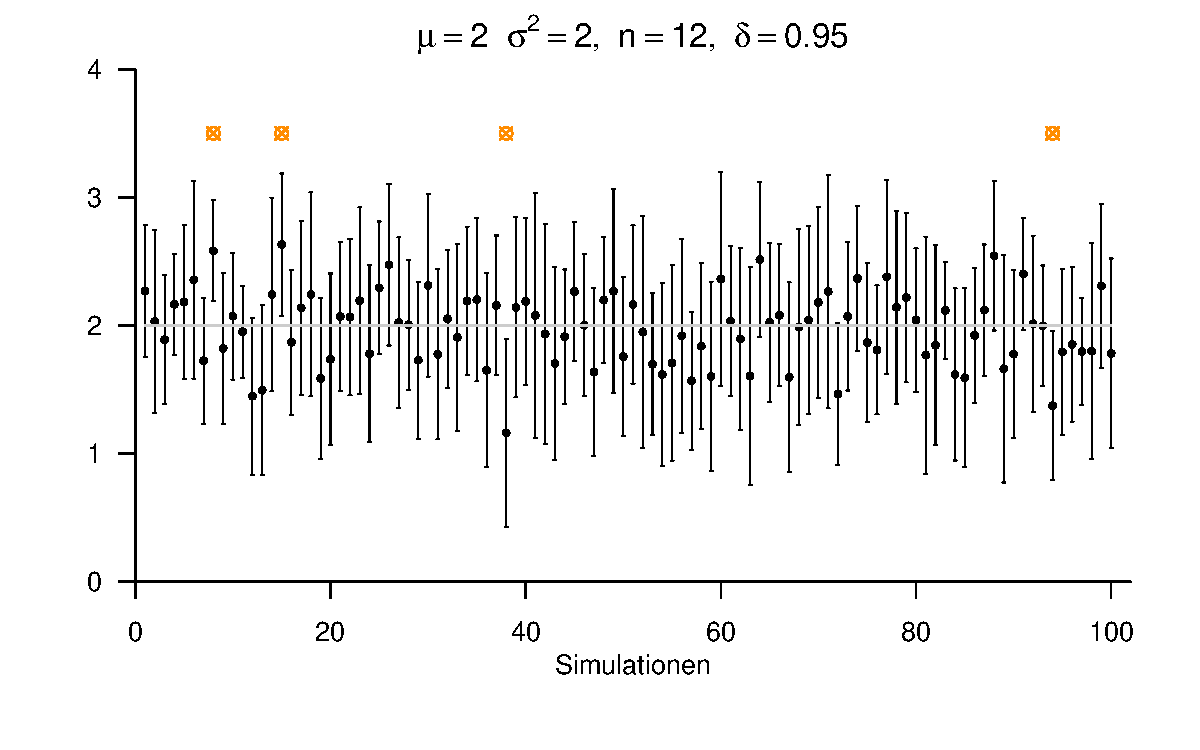
\includegraphics[width=0.9\linewidth]{11_Abbildungen/wtfi_11_ki_normal_sigsqr_unbekannt} \end{center}
\end{frame}

\begin{frame}[fragile]{Konfidenzintervall für den
Erwartungswertparameter der Normalverteilung}
\protect\hypertarget{konfidenzintervall-fuxfcr-den-erwartungswertparameter-der-normalverteilung-8}{}
\noindent(5) Definition des Konfidenzintervalls (fortgeführt)

\small

Simulation der zweiten Interpretation eines Konfidenzintervalls
\vspace{2mm}

\setstretch{1}
\footnotesize

\begin{Shaded}
\begin{Highlighting}[]
\CommentTok{\# Anzahl Simulationen mit \textbackslash{}theta\_1, \textbackslash{}theta\_2,...}
\FunctionTok{set.seed}\NormalTok{(}\DecValTok{2}\NormalTok{)                                        }\CommentTok{\# random number generator seed}
\NormalTok{ns      }\OtherTok{=} \FloatTok{1e2}                                      \CommentTok{\# Anzahl Simulationen}

\CommentTok{\# Modellformulierung}
\NormalTok{mu      }\OtherTok{=} \DecValTok{2} \SpecialCharTok{*} \FunctionTok{seq}\NormalTok{(}\DecValTok{0}\NormalTok{,}\DecValTok{1}\NormalTok{,}\AttributeTok{len =}\NormalTok{ ns)                    }\CommentTok{\# w.a.u. Erwartungswertparameter}
\NormalTok{sigsqr  }\OtherTok{=} \DecValTok{1}                                        \CommentTok{\# w.a.u. Varianzparameter}
\NormalTok{sigma   }\OtherTok{=} \FunctionTok{sqrt}\NormalTok{(sigsqr)                             }\CommentTok{\# w.a.u. St.Abweichungsparameter}
\NormalTok{n       }\OtherTok{=} \DecValTok{12}                                       \CommentTok{\# Stichprobengroesse}
\NormalTok{delta   }\OtherTok{=} \FloatTok{0.95}                                     \CommentTok{\# Konfidenzbedingung}
\NormalTok{t\_delta }\OtherTok{=} \FunctionTok{qt}\NormalTok{((}\DecValTok{1}\SpecialCharTok{+}\NormalTok{delta)}\SpecialCharTok{/}\DecValTok{2}\NormalTok{,n}\DecValTok{{-}1}\NormalTok{)                      }\CommentTok{\# \textbackslash{}Psi\^{}{-}1((\textbackslash{}delta + 1)/2, n{-}1)}

\CommentTok{\# Simulation}
\NormalTok{y\_bar   }\OtherTok{=} \FunctionTok{rep}\NormalTok{(}\ConstantTok{NaN}\NormalTok{,ns)                              }\CommentTok{\# Stichprobenmittelarray}
\NormalTok{S       }\OtherTok{=} \FunctionTok{rep}\NormalTok{(}\ConstantTok{NaN}\NormalTok{,ns)                              }\CommentTok{\# St.Abweichungsarray}
\NormalTok{kappa   }\OtherTok{=} \FunctionTok{matrix}\NormalTok{(}\FunctionTok{rep}\NormalTok{(}\ConstantTok{NaN}\NormalTok{,}\DecValTok{2}\SpecialCharTok{*}\NormalTok{ns), }\AttributeTok{ncol =} \DecValTok{2}\NormalTok{)          }\CommentTok{\# Konfidenzintervallarray}
\ControlFlowTok{for}\NormalTok{(i }\ControlFlowTok{in} \DecValTok{1}\SpecialCharTok{:}\NormalTok{ns)\{}
\NormalTok{   y          }\OtherTok{=} \FunctionTok{rnorm}\NormalTok{(n,mu[i],sigma)               }\CommentTok{\# Stichprobenrealisierung}
\NormalTok{   y\_bar[i]   }\OtherTok{=} \FunctionTok{mean}\NormalTok{(y)                            }\CommentTok{\# Stichprobenmittel}
\NormalTok{   S[i]       }\OtherTok{=} \FunctionTok{sd}\NormalTok{(y)                              }\CommentTok{\# Stichprobenstandardabweichung}
\NormalTok{   kappa[i,}\DecValTok{1}\NormalTok{] }\OtherTok{=}\NormalTok{ y\_bar[i] }\SpecialCharTok{{-}}\NormalTok{ (S[i]}\SpecialCharTok{/}\FunctionTok{sqrt}\NormalTok{(n))}\SpecialCharTok{*}\NormalTok{t\_delta  }\CommentTok{\# untere KI Grenze}
\NormalTok{   kappa[i,}\DecValTok{2}\NormalTok{] }\OtherTok{=}\NormalTok{ y\_bar[i] }\SpecialCharTok{+}\NormalTok{ (S[i]}\SpecialCharTok{/}\FunctionTok{sqrt}\NormalTok{(n))}\SpecialCharTok{*}\NormalTok{t\_delta  }\CommentTok{\# obere KI Grenze}
\NormalTok{\}}
\end{Highlighting}
\end{Shaded}
\end{frame}

\begin{frame}{Konfidenzintervall für den Erwartungswertparameter der
Normalverteilung}
\protect\hypertarget{konfidenzintervall-fuxfcr-den-erwartungswertparameter-der-normalverteilung-9}{}
\noindent(5) Definition des Konfidenzintervalls (fortgeführt)

\small

Simulation der zweiten Interpretation eines Konfidenzintervalls

\vspace{3mm}

\begin{center}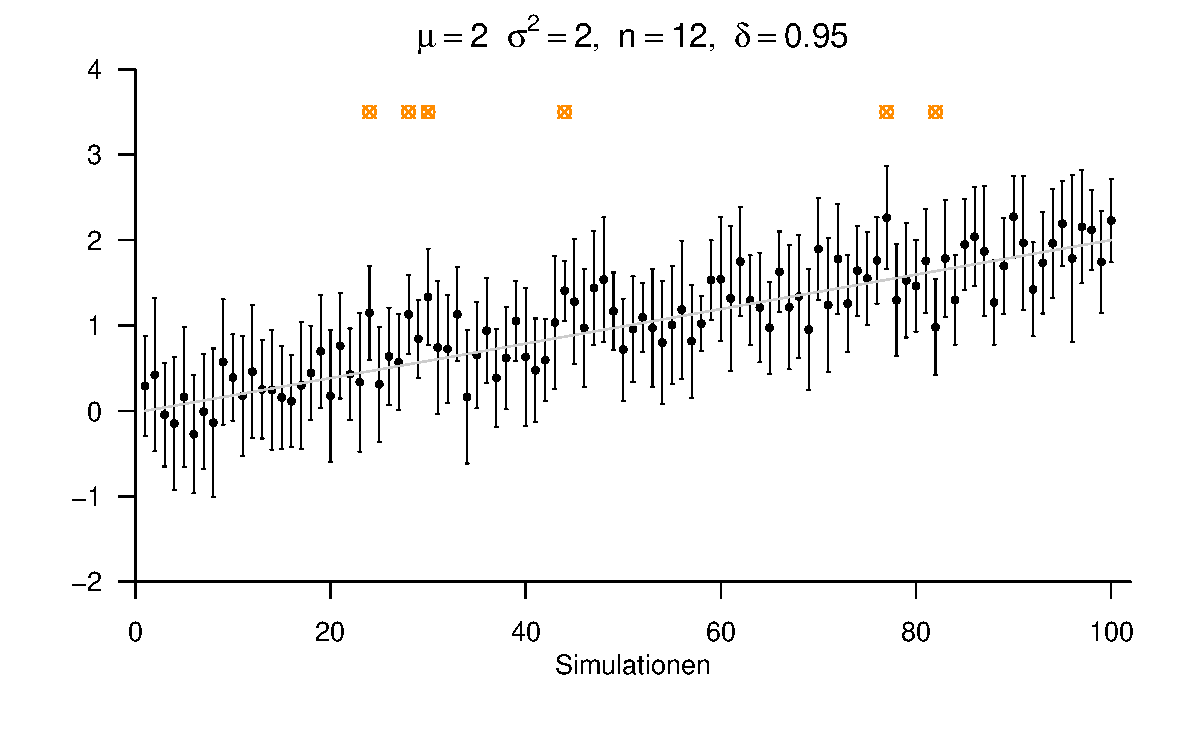
\includegraphics[width=0.9\linewidth]{11_Abbildungen/wtfi_11_ki_normal_sigsqr_unbekannt_mu_variabel} \end{center}
\end{frame}

\begin{frame}{}
\protect\hypertarget{section-8}{}
\setstretch{2.7}
\large

Definition

Konfidenzintervall für den Erwartungswertparameter der Normalverteilung

\textbf{Konfidenzintervall für den Varianzparameter der
Normalverteilung}

Anwendungsbeispiel

Selbstkontrollfragen
\end{frame}

\begin{frame}{Konfidenzintervall für den Varianzparameter der
Normalverteilung}
\protect\hypertarget{konfidenzintervall-fuxfcr-den-varianzparameter-der-normalverteilung}{}
\noindent (1) Definition des statistischen Modells

\small

Es sei \(\ups_1,...,\ups_n \sim N(\mu,\sigma^2)\) eine Stichprobe mit
unbekanntem Varianzparameter \(\sigma^2 > 0\) und bekanntem oder
unbekanntem Erwartungswertparameter \(\mu\). Wir entwickeln ein
\(\delta\)-Konfidenzintervall für den Varianzparameter \(\sigma^2\).

\normalsize

\noindent (2) Definition der Statistik

\small

Wir betrachten die \(U\)-Konfidenzintervallstatistik \begin{equation}
U := \frac{n-1}{\sigma^2}S^2 \mbox{ mit } S^2 := \frac{1}{n-1}\sum_{i=1}^n \left(\ups_i - \bar{\ups}\right)^2.
\end{equation}

\normalsize

\noindent (3) Analyse der Verteilung der Konfidenzintervallstatistik

\small

Für die \(U\)-Konfidenzintervallstatistik gilt \(U \sim \chi^2(n-1)\).
Für einen Beweis dieser Tatsache verweisen wir auf Casella and Berger
(2012), Abschnitt 5.3. Die \(U\)-Konfidenzintervallstatistik ist eine
Funktion von \(\ups_1,...,\ups_n\) (via \(S^2\)) und \(\sigma^2\),
während ihre Verteilung nicht von \(\sigma^2\) abhängt. Wir bezeichnen
die WDF einer \(\chi^2\)-verteilten Zufallvariable mit \(\chi^2\), die
KVF einer \(\chi^2\)-verteilten Zufallvariable mit \(\Xi\) und die
inverse KVF einer \(\chi^2\)-verteilten Zufallvariable mit \(\Xi^{-1}\).
\end{frame}

\begin{frame}[fragile]{(2) Konfidenzintervall für den Varianzparameter
der Normalverteilung}
\protect\hypertarget{konfidenzintervall-fuxfcr-den-varianzparameter-der-normalverteilung-1}{}
\normalsize

\noindent (3) Analyse der Verteilung der Konfidenzintervallstatistik
(fortgeführt) \vspace{2mm}

\tiny
\setstretch{1}

\begin{Shaded}
\begin{Highlighting}[]
\CommentTok{\# Modellformulierung}
\NormalTok{mu      }\OtherTok{=} \DecValTok{10}                                    \CommentTok{\# wahrer Erwartungswertparameter}
\NormalTok{sigsqr  }\OtherTok{=} \DecValTok{4}                                     \CommentTok{\# wahrer bekannter Varianzparameter}
\NormalTok{n       }\OtherTok{=} \DecValTok{12}                                    \CommentTok{\# Stichprobengroesse}
\NormalTok{ns      }\OtherTok{=} \FloatTok{1e4}                                   \CommentTok{\# Anzahl Stichprobenrealisierungen}
\NormalTok{res     }\OtherTok{=} \FloatTok{1e3}                                   \CommentTok{\# Ausgangsraumaufloesung}

\CommentTok{\# analytische Definitionen und Resultate}
\NormalTok{y\_1     }\OtherTok{=} \FunctionTok{seq}\NormalTok{(}\DecValTok{3}\NormalTok{,}\DecValTok{17}\NormalTok{,}\AttributeTok{len =}\NormalTok{ res)                   }\CommentTok{\# y\_1 Raum}
\NormalTok{y\_bar   }\OtherTok{=} \FunctionTok{seq}\NormalTok{(}\DecValTok{3}\NormalTok{,}\DecValTok{17}\NormalTok{,}\AttributeTok{len =}\NormalTok{ res)                   }\CommentTok{\# y\_bar Raum}
\NormalTok{u\_1     }\OtherTok{=} \FunctionTok{seq}\NormalTok{(}\DecValTok{0}\NormalTok{,}\DecValTok{30}\NormalTok{,}\AttributeTok{len =}\NormalTok{ res)                   }\CommentTok{\# normalisierte S\^{}2 Raum}
\NormalTok{p\_y\_1   }\OtherTok{=} \FunctionTok{dnorm}\NormalTok{(y\_1,mu,}\FunctionTok{sqrt}\NormalTok{(sigsqr))            }\CommentTok{\# y\_1 WDF}
\NormalTok{p\_y\_bar }\OtherTok{=} \FunctionTok{dnorm}\NormalTok{(y\_bar,mu,}\FunctionTok{sqrt}\NormalTok{(sigsqr}\SpecialCharTok{/}\NormalTok{n))        }\CommentTok{\# y\_bar WDF}
\NormalTok{p\_u     }\OtherTok{=} \FunctionTok{dchisq}\NormalTok{(u\_1,n}\DecValTok{{-}1}\NormalTok{)                       }\CommentTok{\# u\_1 WDF}

\CommentTok{\# Simulation}
\NormalTok{y\_i     }\OtherTok{=} \FunctionTok{rep}\NormalTok{(}\ConstantTok{NaN}\NormalTok{,ns)                           }\CommentTok{\# y\_1 Array}
\NormalTok{y\_bar   }\OtherTok{=} \FunctionTok{rep}\NormalTok{(}\ConstantTok{NaN}\NormalTok{,ns)                           }\CommentTok{\# \textbackslash{}bar\{y\} Array}
\NormalTok{S\_sqr   }\OtherTok{=} \FunctionTok{rep}\NormalTok{(}\ConstantTok{NaN}\NormalTok{,ns)                           }\CommentTok{\# S\^{}2 Array}
\NormalTok{U       }\OtherTok{=} \FunctionTok{rep}\NormalTok{(}\ConstantTok{NaN}\NormalTok{,ns)                           }\CommentTok{\# U Array}

\ControlFlowTok{for}\NormalTok{(s }\ControlFlowTok{in} \DecValTok{1}\SpecialCharTok{:}\NormalTok{ns)\{                                 }\CommentTok{\# Simulationsiterationen}
\NormalTok{  y         }\OtherTok{=} \FunctionTok{rnorm}\NormalTok{(n,mu,}\FunctionTok{sqrt}\NormalTok{(sigsqr))          }\CommentTok{\# Stichprobenrealisierung}
\NormalTok{  y\_i[s]    }\OtherTok{=}\NormalTok{ y[}\DecValTok{1}\NormalTok{]                              }\CommentTok{\# \textbackslash{}ups\_i}
\NormalTok{  y\_bar[s]  }\OtherTok{=} \FunctionTok{mean}\NormalTok{(y)                           }\CommentTok{\# Stichprobenmittelrealisierung}
\NormalTok{  S\_sqr[s]  }\OtherTok{=} \FunctionTok{var}\NormalTok{(y)                            }\CommentTok{\# Stichprobenvarianzrealisierung}

  \CommentTok{\# U{-}Statistik Realisiation}
\NormalTok{  U[s]      }\OtherTok{=}\NormalTok{ ((n}\DecValTok{{-}1}\NormalTok{)}\SpecialCharTok{/}\NormalTok{sigsqr)}\SpecialCharTok{*}\NormalTok{S\_sqr[s]}
\NormalTok{\}}
\end{Highlighting}
\end{Shaded}
\end{frame}

\begin{frame}{\small Konfidenzintervall für den Varianzparameter der
Normalverteilung}
\protect\hypertarget{konfidenzintervall-fuxfcr-den-varianzparameter-der-normalverteilung-2}{}
\normalsize

\noindent (3) Analyse der Verteilung der Konfidenzintervallstatistik
(fortgeführt)

\vspace{1mm}

\begin{center}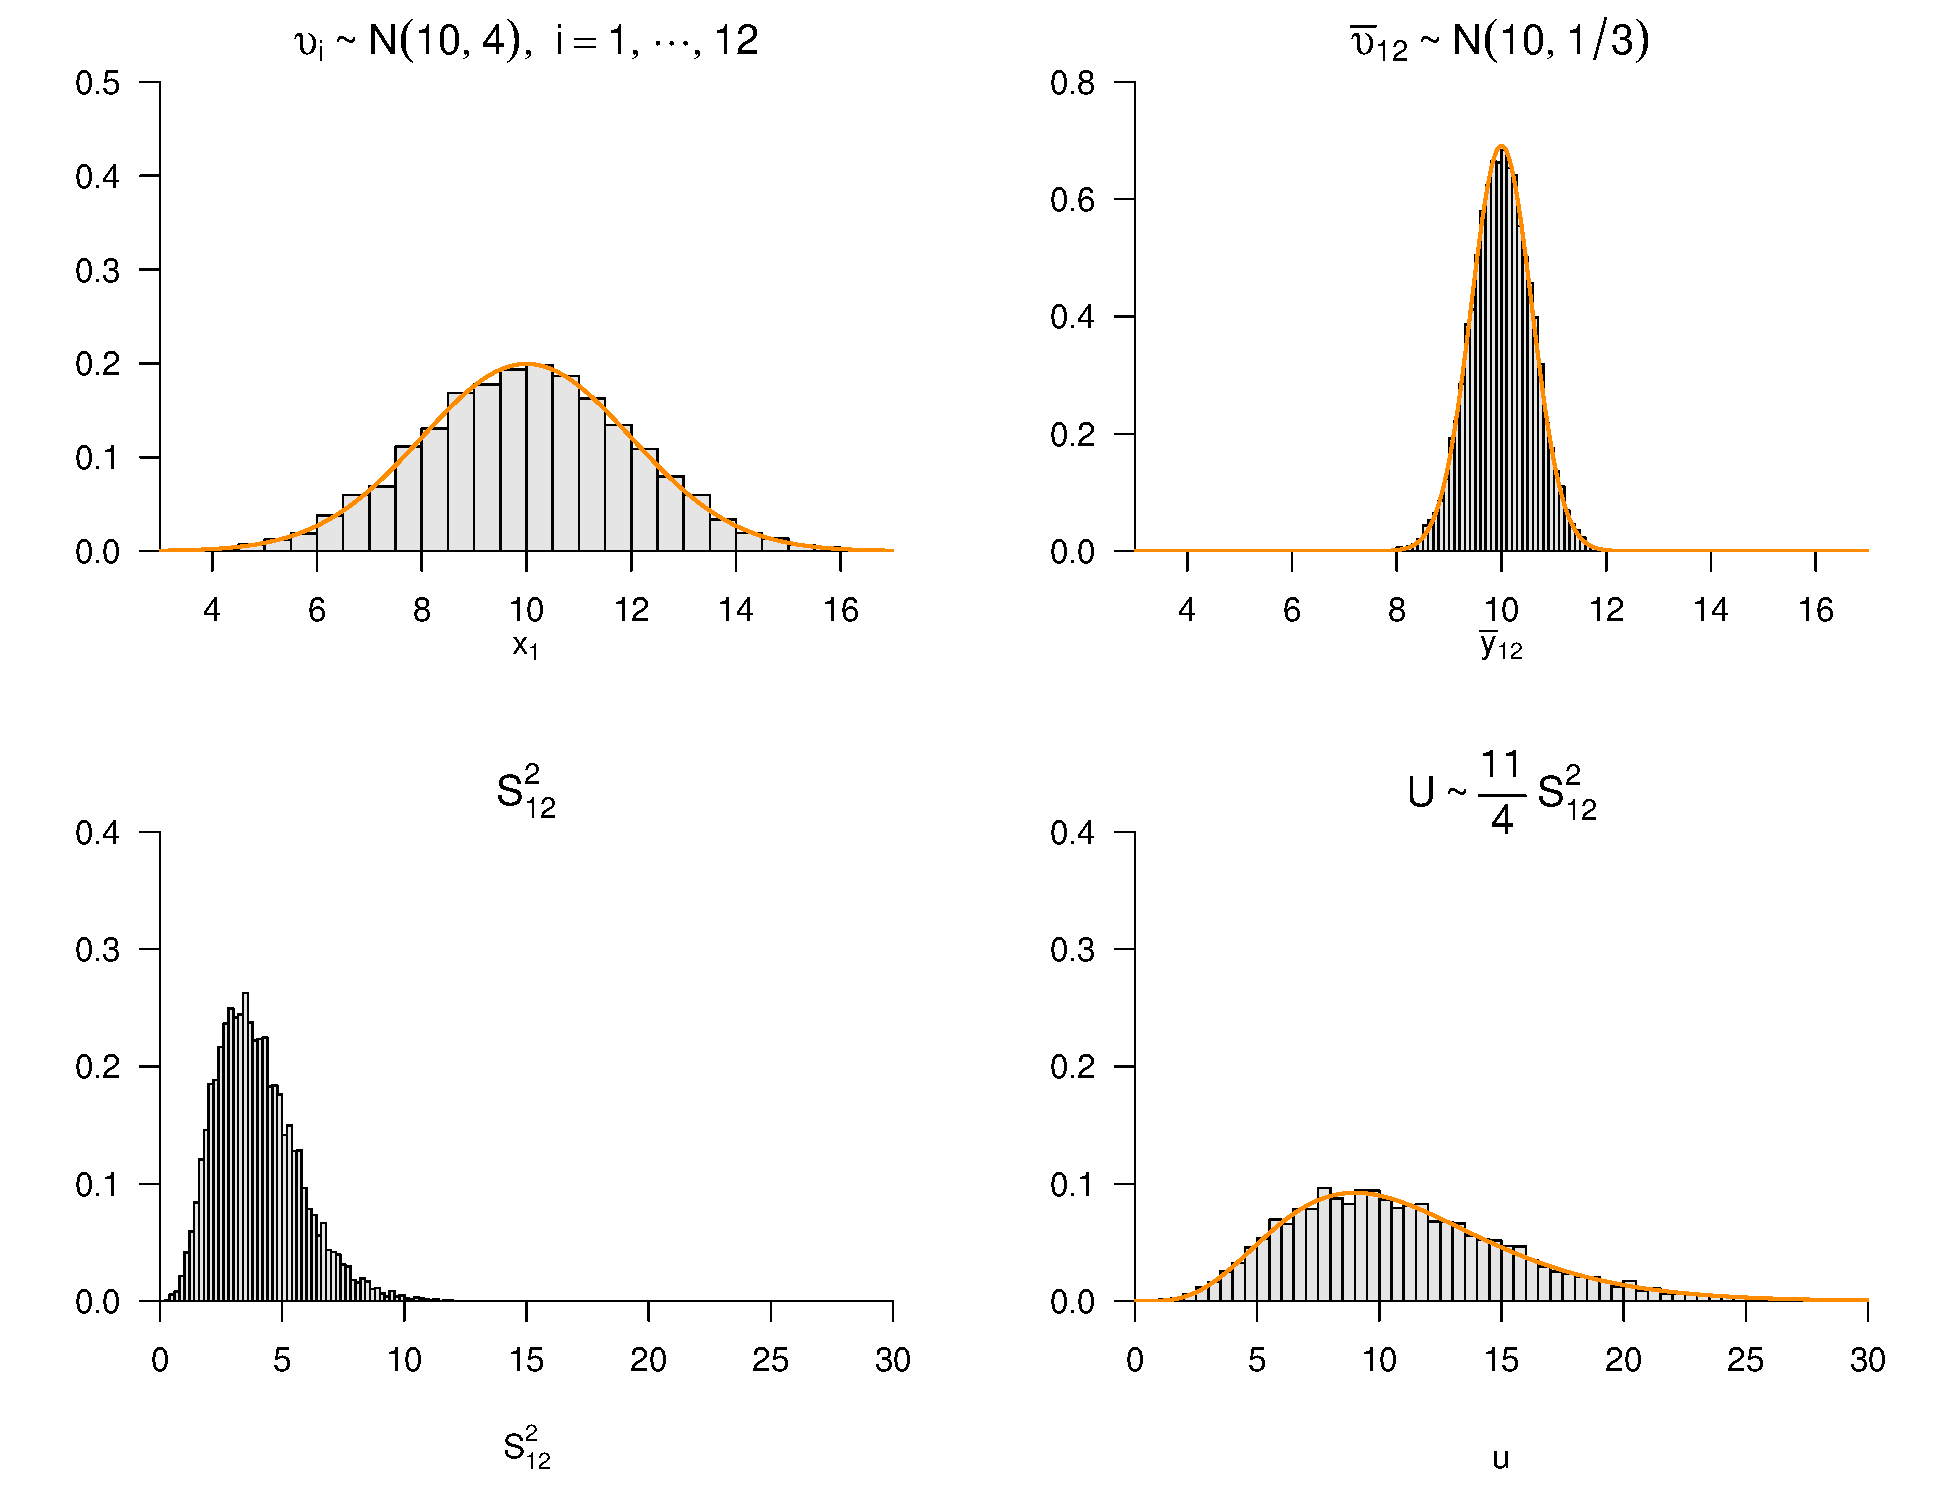
\includegraphics[width=0.8\linewidth]{11_Abbildungen/wtfi_11_u_statistik} \end{center}
\end{frame}

\begin{frame}{Konfidenzintervall für den Varianzparameter der
Normalverteilung}
\protect\hypertarget{konfidenzintervall-fuxfcr-den-varianzparameter-der-normalverteilung-3}{}
\noindent (4) Etablierung der Konfidenzbedingung

\small

Für \(\delta \in ]0,1[\) seien \begin{equation}
\xi_1 := \Xi^{-1}\left(\frac{1 - \delta}{2}; n -1  \right)
\mbox{ und }
\xi_2 := \Xi^{-1}\left(\frac{1 + \delta}{2};n-1 \right)
\end{equation} Es gilt dann \((1 + \delta)/2 - (1 - \delta)/2 = \delta\)
gilt und zum Beispiel gilt für \(n = 10\) und \(\delta = 0.95\),
\(\xi_1 := \Xi^{-1}\left(0.025;9 \right) = 2.70\) und
\(\xi_2 := \Xi^{-1}\left(0.975; 9 \right) = 19.0\). Es gilt hier also
per Definition
\(\mathbb{P}\left(\xi_1 \le U \le \xi_2 \right) = \delta\).

\vspace{2mm}

\begin{center}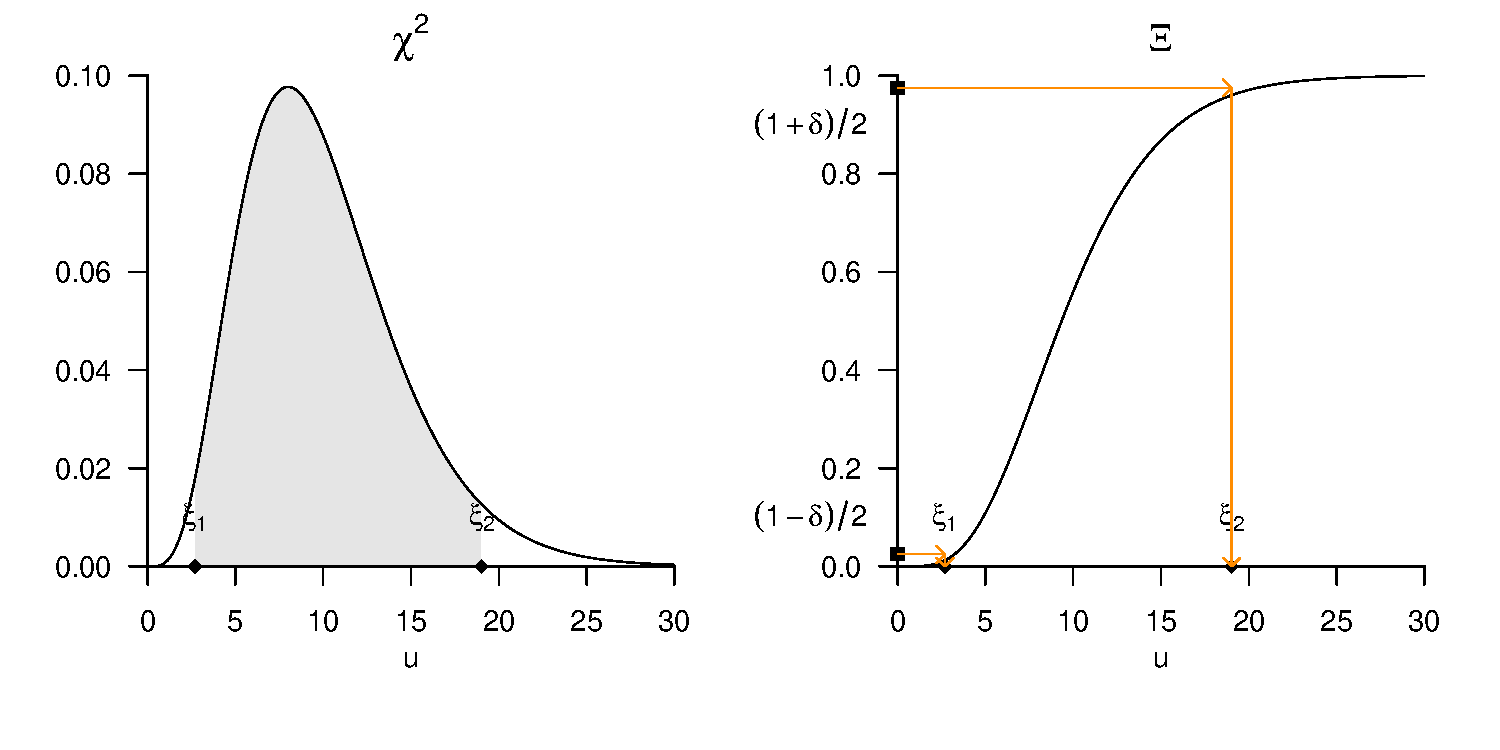
\includegraphics[width=0.8\linewidth]{11_Abbildungen/wtfi_11_ki_u_konfidenzbedingung} \end{center}
\end{frame}

\begin{frame}{Konfidenzintervall für den Varianzparameter der
Normalverteilung}
\protect\hypertarget{konfidenzintervall-fuxfcr-den-varianzparameter-der-normalverteilung-4}{}
\noindent (4) Etablierung der Konfidenzbedingung (fortgeführt)

\small

Mit der Definition von \(\xi_1\) und \(\xi_2\) wie oben folgt dann aber
\footnotesize \begin{align}
\begin{split}
\delta
& = \mathbb{P}\left(\xi_1 \le U \le \xi_2 \right)                                                           \\
& = \mathbb{P}\left(\xi_1 \le \frac{n-1}{\sigma^2}S^2  \le \xi_2 \right)                                    \\
& = \mathbb{P}\left(\xi_1^{-1} \ge \frac{\sigma^2}{(n-1)S^2} \ge \xi_2^{-1} \right)                         \\
& = \mathbb{P}\left(\frac{(n-1)S^2}{\xi_1} \ge \sigma^2 \ge \frac{(n-1)S^2}{\xi_2} \right)              \\
& = \mathbb{P}\left(\frac{(n-1)S^2}{\xi_2} \le \sigma^2 \le \frac{(n-1)S^2)}{\xi_1} \right)             \\
& = \mathbb{P}\left(\left[\frac{(n-1)S^2}{\xi_2}, \frac{(n-1)S^2)}{\xi_1}\right] \ni \sigma^2 \right).  \\
\end{split}
\end{align}

\small

Wir können nun das gesuchte Konfidenzintervall definieren.
\end{frame}

\begin{frame}{\small Beispiel (2) Konfidenzintervall für den
Varianzparameter der Normalverteilung}
\protect\hypertarget{beispiel-2-konfidenzintervall-fuxfcr-den-varianzparameter-der-normalverteilung}{}
\noindent(5) Definition des Konfidenzintervalls \small

Es sei \(\ups_1,...,\ups_n \sim N(\mu,\sigma^2)\) eine Stichprobe mit
unbekanntem Varianzparameter \(\sigma^2\) und bekanntem oder unbekanntem
Erwartungswertparamter \(\mu\) und es seien weiterhin
\(\delta \in ]0,1[\) sowie \begin{equation}
\xi_1 := \Xi^{-1}\left(\frac{1 - \delta}{2};n-1 \right) \mbox{ und }
\xi_2 := \Xi^{-1}\left(\frac{1 + \delta}{2};n-1 \right). 
\end{equation} Definiere \begin{equation}
\kappa := \left[\frac{(n-1)S^2}{\xi_2}, \frac{(n-1)S^2}{\xi_1}\right].
\end{equation} Dann gilt wie oben gezeigt \begin{equation}
\mathbb{P}(\kappa \ni \sigma^2) = \delta.
\end{equation} Damit ist \(\kappa\) ein \(\delta\)-Konfidenzintervall
für \(\sigma^2\).

Man beachte, dass \(\kappa\) ein zufälliges Intervall ist, weil \(S^2\)
eine Zufallsvariable ist.
\end{frame}

\begin{frame}[fragile]{(2) Konfidenzintervall für den Varianzparameter
der Normalverteilung}
\protect\hypertarget{konfidenzintervall-fuxfcr-den-varianzparameter-der-normalverteilung-5}{}
\noindent(5) Definition des Konfidenzintervalls (fortgeführt)

\small

Simulation \vspace{2mm}

\setstretch{1}
\footnotesize

\begin{Shaded}
\begin{Highlighting}[]
\CommentTok{\# Modellformulierung}
\FunctionTok{set.seed}\NormalTok{(}\DecValTok{1}\NormalTok{)                                 }\CommentTok{\# random number generator seed}
\NormalTok{mu      }\OtherTok{=} \DecValTok{2}                                 \CommentTok{\# w.a.u. Erwartungswertparameter}
\NormalTok{sigsqr  }\OtherTok{=} \DecValTok{2}                                 \CommentTok{\# w.a.u. Varianzparameter}
\NormalTok{n       }\OtherTok{=} \DecValTok{12}                                \CommentTok{\# Stichprobengroesse}
\NormalTok{delta   }\OtherTok{=} \FloatTok{0.95}                              \CommentTok{\# Konfidenzbedingung}
\NormalTok{xi\_1    }\OtherTok{=} \FunctionTok{qchisq}\NormalTok{((}\DecValTok{1}\SpecialCharTok{{-}}\NormalTok{delta)}\SpecialCharTok{/}\DecValTok{2}\NormalTok{, n }\SpecialCharTok{{-}} \DecValTok{1}\NormalTok{)        }\CommentTok{\# \textbackslash{}Xi\^{}2((1{-}\textbackslash{}delta)/2; n {-} 1)}
\NormalTok{xi\_2    }\OtherTok{=} \FunctionTok{qchisq}\NormalTok{((}\DecValTok{1}\SpecialCharTok{+}\NormalTok{delta)}\SpecialCharTok{/}\DecValTok{2}\NormalTok{, n }\SpecialCharTok{{-}} \DecValTok{1}\NormalTok{)        }\CommentTok{\# \textbackslash{}Xi\^{}2((1+\textbackslash{}delta)/2; n {-} 1)}

\CommentTok{\# Simulation}
\NormalTok{ns      }\OtherTok{=} \FloatTok{1e2}                               \CommentTok{\# Anzahl Simulationen}
\NormalTok{y\_bar   }\OtherTok{=} \FunctionTok{rep}\NormalTok{(}\ConstantTok{NaN}\NormalTok{,ns)                       }\CommentTok{\# Stichprobenmittelarray}
\NormalTok{S2      }\OtherTok{=} \FunctionTok{rep}\NormalTok{(}\ConstantTok{NaN}\NormalTok{,ns)                       }\CommentTok{\# Stichprobenvarianzarray}
\NormalTok{kappa   }\OtherTok{=} \FunctionTok{matrix}\NormalTok{(}\FunctionTok{rep}\NormalTok{(}\ConstantTok{NaN}\NormalTok{,}\DecValTok{2}\SpecialCharTok{*}\NormalTok{ns), }\AttributeTok{ncol =} \DecValTok{2}\NormalTok{)   }\CommentTok{\# Konfidenzintervallarray}
\ControlFlowTok{for}\NormalTok{(i }\ControlFlowTok{in} \DecValTok{1}\SpecialCharTok{:}\NormalTok{ns)\{                             }\CommentTok{\# Simulationsiterationen}
\NormalTok{   y        }\OtherTok{=} \FunctionTok{rnorm}\NormalTok{(n,mu,}\FunctionTok{sqrt}\NormalTok{(sigsqr))      }\CommentTok{\# Stichprobenrealisierung}
\NormalTok{   S2[i]    }\OtherTok{=} \FunctionTok{var}\NormalTok{(y)                        }\CommentTok{\# Stichprobenvarianz}
\NormalTok{   kappa[i,}\DecValTok{1}\NormalTok{]   }\OtherTok{=}\NormalTok{ (n}\DecValTok{{-}1}\NormalTok{)}\SpecialCharTok{*}\NormalTok{S2[i]}\SpecialCharTok{/}\NormalTok{xi\_2          }\CommentTok{\# untere KI Grenze}
\NormalTok{   kappa[i,}\DecValTok{2}\NormalTok{]   }\OtherTok{=}\NormalTok{ (n}\DecValTok{{-}1}\NormalTok{)}\SpecialCharTok{*}\NormalTok{S2[i]}\SpecialCharTok{/}\NormalTok{xi\_1          }\CommentTok{\# obere KI Grenze}
\NormalTok{\}}
\end{Highlighting}
\end{Shaded}
\end{frame}

\begin{frame}{\small Beispiel (2) Konfidenzintervall für den
Varianzparameter der Normalverteilung}
\protect\hypertarget{beispiel-2-konfidenzintervall-fuxfcr-den-varianzparameter-der-normalverteilung-1}{}
\noindent(5) Definition des Konfidenzintervalls (fortgeführt)

\small

Simulation

\vspace{3mm}

\begin{center}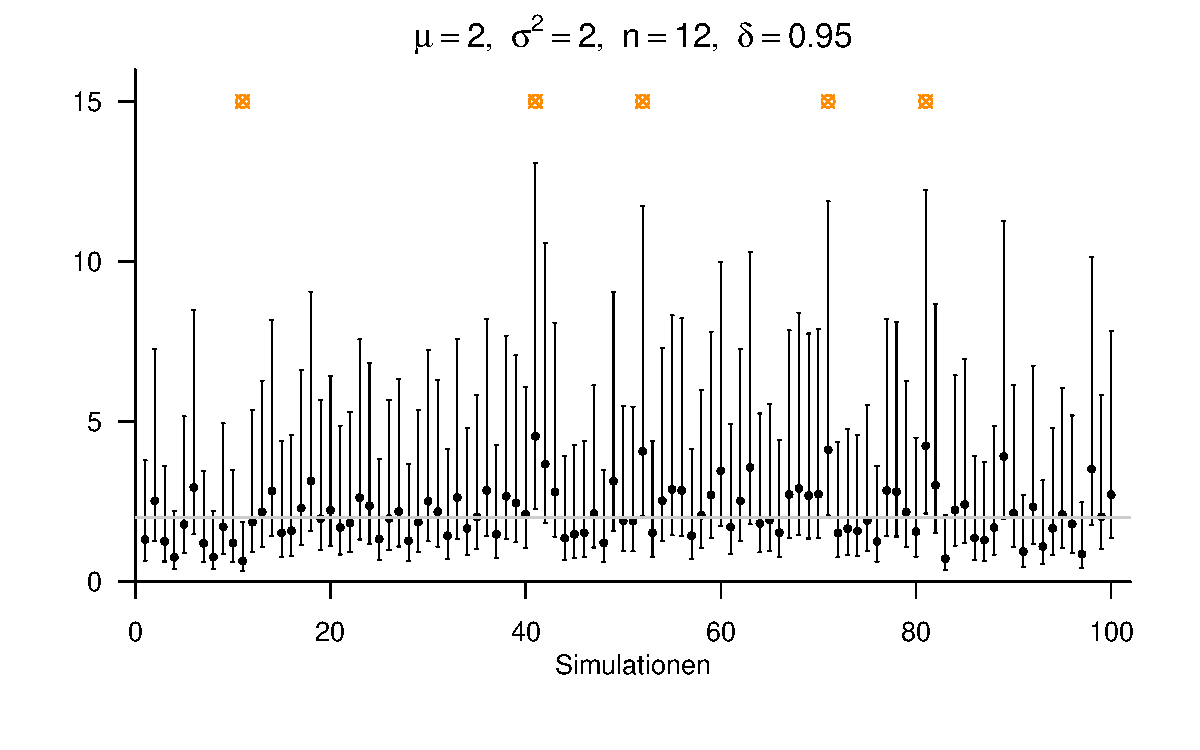
\includegraphics[width=0.9\linewidth]{11_Abbildungen/wtfi_11_ki_sigsqr} \end{center}
\end{frame}

\begin{frame}{}
\protect\hypertarget{section-9}{}
\setstretch{2.7}
\large

Definition

Konfidenzintervall für den Erwartungswertparameter der Normalverteilung

Konfidenzintervall für den Varianzparameter der Normalverteilung

\textbf{Anwendungsbeispiel}

Selbstkontrollfragen
\end{frame}

\begin{frame}[t]{Anwendungsbeispiel}
\protect\hypertarget{anwendungsbeispiel}{}
Beispiel \textbar{} Evidenzbasierte Evaluation von Psychotherapie bei
Depression

\begin{center}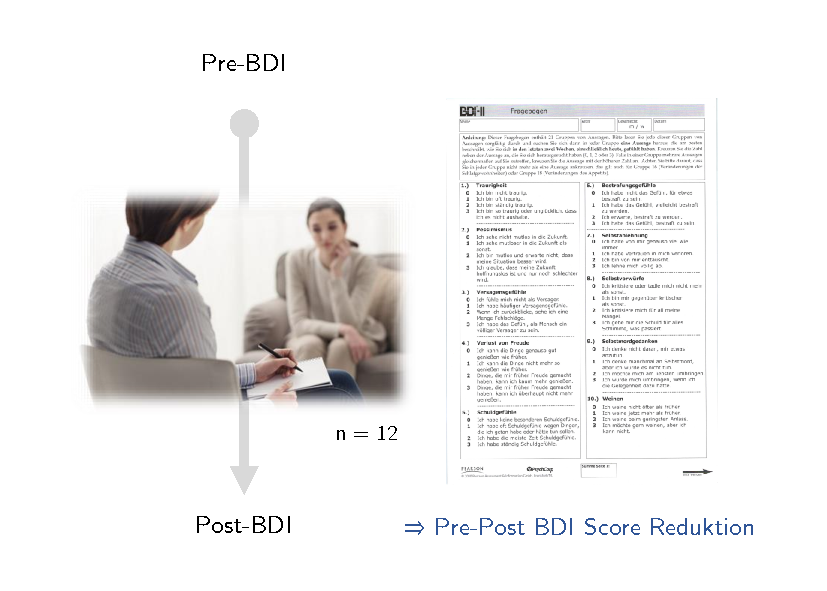
\includegraphics[width=0.9\linewidth]{11_Abbildungen/wtfi_11_messplan} \end{center}
\end{frame}

\begin{frame}[fragile,t]{Anwendungsbeispiel}
\protect\hypertarget{anwendungsbeispiel-1}{}
Beispiel \textbar{} Evidenzbasierte Evaluation von Psychotherapie bei
Depression

\small
\vspace{2mm}

\footnotesize

\begin{Shaded}
\begin{Highlighting}[]
\NormalTok{fname }\OtherTok{=} \FunctionTok{file.path}\NormalTok{(}\FunctionTok{getwd}\NormalTok{(), }\StringTok{"11\_Konfidenzintervalle.csv"}\NormalTok{)}
\NormalTok{D     }\OtherTok{=} \FunctionTok{read.table}\NormalTok{(fname, }\AttributeTok{sep =} \StringTok{","}\NormalTok{, }\AttributeTok{header =}\NormalTok{ T)}
\end{Highlighting}
\end{Shaded}

\vspace{2mm}

\begin{longtable}[]{@{}rr@{}}
\toprule()
i & BDI.Reduktion \\
\midrule()
\endhead
1 & -1 \\
2 & 3 \\
3 & -2 \\
4 & 9 \\
5 & 3 \\
6 & -2 \\
7 & 4 \\
8 & 5 \\
9 & 5 \\
10 & 1 \\
11 & 9 \\
12 & 4 \\
\bottomrule()
\end{longtable}
\end{frame}

\begin{frame}[t]{Anwendungsbeispiel}
\protect\hypertarget{anwendungsbeispiel-2}{}
Beispiel \textbar{} Evidenzbasierte Evaluation von Psychotherapie bei
Depression \vspace{2mm}

\small

Für die Pre-Post BDI Score Reduktion \(\ups_i\) der \(i\)ten von \(n\)
Patient:innen legen wir das Modell \begin{equation}
\ups_{i} = \mu + \varepsilon_{i} \mbox{ mit } \varepsilon_{i} \sim N(0,\sigma^2) \mbox{ u.i.v. für } i = 1,...,n
\end{equation} zugrunde. Dabei wird die Pre-Post BDI Reduktion
\(\ups_i\) der \(i\)ten Patient:in also mithilfe einer über die Gruppe
von Patient:innen identischen Pre-Post BDI Score Reduktion
\(\mu \in \mathbb{R}\) und einer Patient:innen-spezifischen
normalverteilten Pre-Post BDI Score Reduktionsabweichung
\(\varepsilon_{i}\) erklärt

Wie gezeigt ist dieses Modell äquivalent zum Normalverteilungsmodell
\begin{equation}
\ups_1,...,\ups_n \sim N(\mu,\sigma^2).
\end{equation}

Die Standardprobleme der Frequentistischen Inferenz führen in diesem
Szenario auf folgende Fragen:

\begin{enumerate}
[(1)]
\tightlist
\item
  Was sind sinnvolle Tipps für die wahren, aber unbekannten,
  Parameterwerte \(\mu\) und \(\sigma^2\)?
\item
  Wie hoch ist im Frequentistischen Sinn die mit diesen Tipps
  assoziierte Unsicherheit?
\item
  Entscheiden wir uns sinnvollerweise für die Hypothese, dass gilt
  \(\mu\neq 0\) ?
\end{enumerate}
\end{frame}

\begin{frame}[fragile,t]{Anwendungsbeispiel}
\protect\hypertarget{anwendungsbeispiel-3}{}
Beispiel \textbar{} Evidenzbasierte Evaluation von Psychotherapie bei
Depression

\vspace{2mm}
\footnotesize

\begin{Shaded}
\begin{Highlighting}[]
\CommentTok{\# Einlesen und Auswahl der Daten}
\NormalTok{fname }\OtherTok{=} \FunctionTok{file.path}\NormalTok{(}\FunctionTok{getwd}\NormalTok{(), }\StringTok{"11\_Konfidenzintervalle.csv"}\NormalTok{)}
\NormalTok{D     }\OtherTok{=} \FunctionTok{read.table}\NormalTok{(fname, }\AttributeTok{sep =} \StringTok{","}\NormalTok{, }\AttributeTok{header =}\NormalTok{ T)}
\NormalTok{y     }\OtherTok{=}\NormalTok{ D}\SpecialCharTok{$}\NormalTok{BDI.Reduktion}
\end{Highlighting}
\end{Shaded}

Wir haben in (10) Parameterschätzung gesehen, dass unverzerrte Schätzer
für den Erwartungswertparameter \(\mu\) und den Varianzparameter
\(\sigma^2\) durch das Stichprobenmittel und die Stichprobenvarianz
gegeben sind.

\vspace{3mm}

\begin{Shaded}
\begin{Highlighting}[]
\NormalTok{mu\_hat     }\OtherTok{=} \FunctionTok{mean}\NormalTok{(y)    }\CommentTok{\# Stichprobenmittel als Erwartungswertparameterschätzer}
\NormalTok{sigsqr\_hat }\OtherTok{=} \FunctionTok{var}\NormalTok{(y)     }\CommentTok{\# Stichprobenvarianz als Varianzparameterschätzer}
\end{Highlighting}
\end{Shaded}

Es sind also \(\hat{\mu} = 3.17\) und \(\hat{\sigma}^{2} = 13.8\)
sinnvolle Tipps für \(\mu\) und \(\sigma^2\) basierend auf den
vorliegenden 12 Datenpunkten.

Um die mit diesen Tipps assoziierte Unsicherheit zu quantifizieren, geht
die Frequentistische Inferenz zur Intervallschätzung mithilfe von
\(\delta\)-Konfidenzintervallen über, für die die assoziierte
Unsicherheit dann ein ein prädefiniertes Level von 1 - \(\delta\) hat.
Im langfristigen Mittel überdeckt ein angegebenes
\(\delta\)-Konfidenzintervall den wahren, aber unbekannten Parameterwert
in (nur) \(1-\delta\cdot\) 100 von 100 Fällen nicht. Für ein großes
\(\delta\) wie \(\delta = 0.95\) ist die mit dieser Intervallschätzung
assoziierte Unsicherheit also mit \(1 - 0.95 = 0.05\) also eher gering.
\end{frame}

\begin{frame}[fragile,t]{Anwendungsbeispiel}
\protect\hypertarget{anwendungsbeispiel-4}{}
Beispiel \textbar{} Evidenzbasierte Evaluation von Psychotherapie bei
Depression \vspace{2mm}

\tiny
\setstretch{1}

\begin{Shaded}
\begin{Highlighting}[]
\CommentTok{\# Konfidenzintervall für den Erwartungswertparameter}
\NormalTok{delta    }\OtherTok{=} \FloatTok{0.95}                                 \CommentTok{\# Konfidenzlevel}
\NormalTok{n        }\OtherTok{=} \FunctionTok{length}\NormalTok{(y)                            }\CommentTok{\# Anzahl Datenpunkte}
\NormalTok{t\_delta  }\OtherTok{=} \FunctionTok{qt}\NormalTok{((}\DecValTok{1}\SpecialCharTok{+}\NormalTok{delta)}\SpecialCharTok{/}\DecValTok{2}\NormalTok{,n}\DecValTok{{-}1}\NormalTok{)                  }\CommentTok{\# \textbackslash{}psi\^{}{-}1((\textbackslash{}delta + 1)/2, n{-}1)}
\NormalTok{y\_bar    }\OtherTok{=} \FunctionTok{mean}\NormalTok{(y)                              }\CommentTok{\# Stichprobenmittel}
\NormalTok{s        }\OtherTok{=} \FunctionTok{sd}\NormalTok{(y)                                }\CommentTok{\# Stichprobenstandardabweichung}
\NormalTok{mu\_hat   }\OtherTok{=}\NormalTok{ y\_bar                                }\CommentTok{\# Erwartungswertparameterschätzer}
\NormalTok{mu\_hat\_u }\OtherTok{=}\NormalTok{ y\_bar }\SpecialCharTok{{-}}\NormalTok{ (s}\SpecialCharTok{/}\FunctionTok{sqrt}\NormalTok{(n))}\SpecialCharTok{*}\NormalTok{t\_delta          }\CommentTok{\# untere KI Grenze}
\NormalTok{mu\_hat\_o }\OtherTok{=}\NormalTok{ y\_bar }\SpecialCharTok{+}\NormalTok{ (s}\SpecialCharTok{/}\FunctionTok{sqrt}\NormalTok{(n))}\SpecialCharTok{*}\NormalTok{t\_delta          }\CommentTok{\# obere  KI Grenze}
\end{Highlighting}
\end{Shaded}

\footnotesize
\setstretch{1.4}

Das 0.95-Konfidenzintervall für den Erwartungswertparameter ist
\([0.80,5.52]\). Im langfristigen Mittel überdeckt so berechnetes
Konfidenzintervall den wahren, aber unbekannten, Erwartungswertparameter
in 95 von 100 Fällen.

\vspace{2mm}

\tiny
\setstretch{1}

\begin{Shaded}
\begin{Highlighting}[]
\CommentTok{\# Konfidenzintervall für den Erwartungswertparameter}
\NormalTok{delta         }\OtherTok{=} \FloatTok{0.95}                            \CommentTok{\# Konfidenzlevel}
\NormalTok{n            }\OtherTok{=} \FunctionTok{length}\NormalTok{(y)                        }\CommentTok{\# Anzahl Datenpunkte}
\NormalTok{xi\_1         }\OtherTok{=} \FunctionTok{qchisq}\NormalTok{((}\DecValTok{1}\SpecialCharTok{{-}}\NormalTok{delta)}\SpecialCharTok{/}\DecValTok{2}\NormalTok{, n }\SpecialCharTok{{-}} \DecValTok{1}\NormalTok{)       }\CommentTok{\# \textbackslash{}Xi\^{}2((1{-}\textbackslash{}delta)/2; n {-} 1)}
\NormalTok{xi\_2         }\OtherTok{=} \FunctionTok{qchisq}\NormalTok{((}\DecValTok{1}\SpecialCharTok{+}\NormalTok{delta)}\SpecialCharTok{/}\DecValTok{2}\NormalTok{, n }\SpecialCharTok{{-}} \DecValTok{1}\NormalTok{)       }\CommentTok{\# \textbackslash{}Xi\^{}2((1+\textbackslash{}delta)/2; n {-} 1)}
\NormalTok{s2           }\OtherTok{=} \FunctionTok{var}\NormalTok{(y)                           }\CommentTok{\# Stichprobenstandardabweichung}
\NormalTok{sigsqr\_hat   }\OtherTok{=}\NormalTok{ s2                               }\CommentTok{\# Varianzparameterschätzer}
\NormalTok{sigsqr\_hat\_u }\OtherTok{=}\NormalTok{ (n}\DecValTok{{-}1}\NormalTok{)}\SpecialCharTok{*}\NormalTok{s2}\SpecialCharTok{/}\NormalTok{xi\_2                    }\CommentTok{\# untere KI Grenze}
\NormalTok{sigsqr\_hat\_o }\OtherTok{=}\NormalTok{ (n}\DecValTok{{-}1}\NormalTok{)}\SpecialCharTok{*}\NormalTok{s2}\SpecialCharTok{/}\NormalTok{xi\_1                    }\CommentTok{\# obere KI Grenze}
\end{Highlighting}
\end{Shaded}

\footnotesize
\setstretch{1.4}

Das 0.95-Konfidenzintervall für den Varianzparameter ist
\([6.91, 39.74]\). Im langfristigen Mittel überdeckt ein so berechnetes
Konfidenzintervall den wahren, aber unbekannten, Varianzparameter in 95
von 100 Fällen.
\end{frame}

\begin{frame}{}
\protect\hypertarget{section-10}{}
\setstretch{2.7}
\large

Definition

Konfidenzintervall für den Erwartungswertparameter der Normalverteilung

Konfidenzintervall für den Varianzparameter der Normalverteilung

Anwendungsbeispiel

\textbf{Selbstkontrollfragen}
\end{frame}

\begin{frame}{Selbstkontrollfragen}
\protect\hypertarget{selbstkontrollfragen}{}
\setstretch{3}
\small

\begin{enumerate}
\tightlist
\item
  Definieren Sie den Begriff des \(\delta\)-Konfidenzintervalls.
\item
  Geben Sie zwei Interpretationen eines \(\delta\)-Konfidenzintervalls.
\item
  Erläutern Sie die typischen Schritte zur Konstruktion eines
  \(\delta\)-Konfidenzintervalls.
\item
  Definieren Sie die \(T\)-Konfidenzintervallstatistik und geben Sie
  ihre Verteilung an.
\item
  Geben Sie das \(\delta\)-Konfidenzintervall für den Erwartungswert der
  Normalverteilung an.
\item
  Definieren Sie die \(U\)-Konfidenzintervallstatistik und geben Sie
  ihre Verteilung an.
\item
  Geben Sie das \(\delta\)-Konfidenzintervall für den Varianzparameter
  der Normalverteilung an.
\end{enumerate}
\end{frame}

\begin{frame}{References}
\protect\hypertarget{references}{}
\footnotesize

\hypertarget{refs}{}
\begin{CSLReferences}{1}{0}
\leavevmode\vadjust pre{\hypertarget{ref-casella_2012}{}}%
Casella, G, and R Berger. 2012. \emph{Statistical {Inference}}.
{Duxbury}.

\end{CSLReferences}
\end{frame}

\end{document}
